%% LyX 2.4.3 created this file.  For more info, see https://www.lyx.org/.
%% Do not edit unless you really know what you are doing.
\documentclass[journal,article,submit,pdftex,moreauthors]{Definitions/mdpi}
\usepackage{textcomp}
\usepackage[utf8]{inputenc}
\usepackage{array}
\usepackage{cprotect}
\usepackage{float}
\usepackage{multirow}
\usepackage{varwidth}
\usepackage{amsmath}
\usepackage{graphicx}
\usepackage{rotfloat}

\makeatletter

%%%%%%%%%%%%%%%%%%%%%%%%%%%%%% LyX specific LaTeX commands.

\Title{The SIOA Algorithm: A Bio-Inspired Approach for Efficient Optimization}

\TitleCitation{The SIOA Algorithm: A Bio-Inspired Approach for Efficient Optimization}

\Author{Vasileios Charilogis$^{1}$, Ioannis G. Tsoulos$^{2,*}$ , Dimitrios
Tsalikakis$^{3}$ and Anna Maria Gianni$^{4}$}

\AuthorNames{Vasileios Charilogis, Ioannis G. Tsoulos, Dimitrios Tsalikakis and
Anna Maria Gianni}

\AuthorCitation{Charilogis, V.; Tsoulos, I.G.;Tsalikakis D.;Gianni A.M.}


\address{$^{1}$\quad{}Department of Informatics and Telecommunications,
University of Ioannina, 47150 Kostaki Artas, Greece; v.charilog@uoi.gr\\
$^{2}$\quad{}Department of Informatics and Telecommunications, University
of Ioannina, 47150 Kostaki Artas, Greece; itsoulos@uoi.gr\\
$^{3}\quad$Department of Engineering Informatics and Telecommunications,
University of Western Macedonia, 50100 Kozani, Greece; tsalikakis@gmail.com\\
$^{4}$\quad{}Department of Informatics and Telecommunications, University
of Ioannina, 47150 Kostaki Artas, Greece; am.gianni@uoi.gr}


\corres{Correspondence: itsoulos@uoi.gr}


\abstract{The Sporulation-Inspired Optimization Algorithm (SIOA) is an innovative
metaheuristic optimization method inspired by the biological mechanisms
of microbial sporulation and dispersal. SIOA operates on a dynamic
population of solutions (“microorganisms”) and alternates between
two main phases: sporulation, where new “spores” are generated through
adaptive random perturbations combined with guided search towards
the global best, and germination, in which these spores are evaluated
and may replace the most similar and less effective individuals in
the population. A distinctive feature of SIOA is its fully self-adaptive
parameter control, as the dispersal radius and the probabilities of
sporulation and germination are automatically adjusted in response
to search progress. The algorithm also integrates a special \textquotedbl zero-reset\textquotedbl{}
mechanism, enhancing its ability to detect global optima located near
the origin. SIOA further incorporates a stochastic local search phase
to refine solutions and accelerate convergence. Experimental results
demonstrate that SIOA achieves high-quality solutions with a reduced
number of function evaluations, especially in complex, multimodal,
or high-dimensional problems. Overall, SIOA provides a robust and
flexible optimization framework, suitable for a wide range of challenging
optimization tasks.}


\keyword{Optimization; SIOA Optimizer; Evolutionary Algorithms; Global Optimization;
Evolutionary Techniques; Metaheuristics;}

\DeclareTextSymbolDefault{\textquotedbl}{T1}
%% Because html converters don't know tabularnewline
\providecommand{\tabularnewline}{\\}
%% Variable width box for table cells
\newenvironment{cellvarwidth}[1][t]
    {\begin{varwidth}[#1]{\linewidth}}
    {\@finalstrut\@arstrutbox\end{varwidth}}
\floatstyle{ruled}
\newfloat{algorithm}{tbp}{loa}
\providecommand{\algorithmname}{Algorithm}
\floatname{algorithm}{\protect\algorithmname}

%%%%%%%%%%%%%%%%%%%%%%%%%%%%%% User specified LaTeX commands.
%  LaTeX support: latex@mdpi.com 
%  For support, please attach all files needed for compiling as well as the log file, and specify your operating system, LaTeX version, and LaTeX editor.

%=================================================================


% For posting an early version of this manuscript as a preprint, you may use "preprints" as the journal and change "submit" to "accept". The document class line would be, e.g., \documentclass[preprints,article,accept,moreauthors,pdftex]{mdpi}. This is especially recommended for submission to arXiv, where line numbers should be removed before posting. For preprints.org, the editorial staff will make this change immediately prior to posting.

%--------------------
% Class Options:
%--------------------
%----------
% journal
%----------
% Choose between the following MDPI journals:
% acoustics, actuators, addictions, admsci, adolescents, aerospace, agriculture, agriengineering, agronomy, ai, algorithms, allergies, alloys, analytica, animals, antibiotics, antibodies, antioxidants, applbiosci, appliedchem, appliedmath, applmech, applmicrobiol, applnano, applsci, aquacj, architecture, arts, asc, asi, astronomy, atmosphere, atoms, audiolres, automation, axioms, bacteria, batteries, bdcc, behavsci, beverages, biochem, bioengineering, biologics, biology, biomass, biomechanics, biomed, biomedicines, biomedinformatics, biomimetics, biomolecules, biophysica, biosensors, biotech, birds, bloods, blsf, brainsci, breath, buildings, businesses, cancers, carbon, cardiogenetics, catalysts, cells, ceramics, challenges, chemengineering, chemistry, chemosensors, chemproc, children, chips, cimb, civileng, cleantechnol, climate, clinpract, clockssleep, cmd, coasts, coatings, colloids, colorants, commodities, compounds, computation, computers, condensedmatter, conservation, constrmater, cosmetics, covid, crops, cryptography, crystals, csmf, ctn, curroncol, currophthalmol, cyber, dairy, data, dentistry, dermato, dermatopathology, designs, diabetology, diagnostics, dietetics, digital, disabilities, diseases, diversity, dna, drones, dynamics, earth, ebj, ecologies, econometrics, economies, education, ejihpe, electricity, electrochem, electronicmat, electronics, encyclopedia, endocrines, energies, eng, engproc, ent, entomology, entropy, environments, environsciproc, epidemiologia, epigenomes, est, fermentation, fibers, fintech, fire, fishes, fluids, foods, forecasting, forensicsci, forests, foundations, fractalfract, fuels, futureinternet, futureparasites, futurepharmacol, futurephys, futuretransp, galaxies, games, gases, gastroent, gastrointestdisord, gels, genealogy, genes, geographies, geohazards, geomatics, geosciences, geotechnics, geriatrics, hazardousmatters, healthcare, hearts, hemato, heritage, highthroughput, histories, horticulturae, humanities, humans, hydrobiology, hydrogen, hydrology, hygiene, idr, ijerph, ijfs, ijgi, ijms, ijns, ijtm, ijtpp, immuno, informatics, information, infrastructures, inorganics, insects, instruments, inventions, iot, j, jal, jcdd, jcm, jcp, jcs, jdb, jeta, jfb, jfmk, jimaging, jintelligence, jlpea, jmmp, jmp, jmse, jne, jnt, jof, joitmc, jor, journalmedia, jox, jpm, jrfm, jsan, jtaer, jzbg, kidney, kidneydial, knowledge, land, languages, laws, life, liquids, literature, livers, logics, logistics, lubricants, lymphatics, machines, macromol, magnetism, magnetochemistry, make, marinedrugs, materials, materproc, mathematics, mca, measurements, medicina, medicines, medsci, membranes, merits, metabolites, metals, meteorology, methane, metrology, micro, microarrays, microbiolres, micromachines, microorganisms, microplastics, minerals, mining, modelling, molbank, molecules, mps, msf, mti, muscles, nanoenergyadv, nanomanufacturing, nanomaterials, ncrna, network, neuroglia, neurolint, neurosci, nitrogen, notspecified, nri, nursrep, nutraceuticals, nutrients, obesities, oceans, ohbm, onco, oncopathology, optics, oral, organics, organoids, osteology, oxygen, parasites, parasitologia, particles, pathogens, pathophysiology, pediatrrep, pharmaceuticals, pharmaceutics, pharmacoepidemiology, pharmacy, philosophies, photochem, photonics, phycology, physchem, physics, physiologia, plants, plasma, pollutants, polymers, polysaccharides, poultry, powders, preprints, proceedings, processes, prosthesis, proteomes, psf, psych, psychiatryint, psychoactives, publications, quantumrep, quaternary, qubs, radiation, reactions, recycling, regeneration, religions, remotesensing, reports, reprodmed, resources, rheumato, risks, robotics, ruminants, safety, sci, scipharm, seeds, sensors, separations, sexes, signals, sinusitis, skins, smartcities, sna, societies, socsci, software, soilsystems, solar, solids, sports, standards, stats, stresses, surfaces, surgeries, suschem, sustainability, symmetry, synbio, systems, taxonomy, technologies, telecom, test, textiles, thalassrep, thermo, tomography, tourismhosp, toxics, toxins, transplantology, transportation, traumacare, traumas, tropicalmed, universe, urbansci, uro, vaccines, vehicles, venereology, vetsci, vibration, viruses, vision, waste, water, wem, wevj, wind, women, world, youth, zoonoticdis 

%---------
% article
%---------
% The default type of manuscript is "article", but can be replaced by: 
% abstract, addendum, article, book, bookreview, briefreport, casereport, comment, commentary, communication, conferenceproceedings, correction, conferencereport, entry, expressionofconcern, extendedabstract, datadescriptor, editorial, essay, erratum, hypothesis, interestingimage, obituary, opinion, projectreport, reply, retraction, review, perspective, protocol, shortnote, studyprotocol, systematicreview, supfile, technicalnote, viewpoint, guidelines, registeredreport, tutorial
% supfile = supplementary materials

%----------
% submit
%----------
% The class option "submit" will be changed to "accept" by the Editorial Office when the paper is accepted. This will only make changes to the frontpage (e.g., the logo of the journal will get visible), the headings, and the copyright information. Also, line numbering will be removed. Journal info and pagination for accepted papers will also be assigned by the Editorial Office.

%------------------
% moreauthors
%------------------
% If there is only one author the class option oneauthor should be used. Otherwise use the class option moreauthors.

%---------
% pdftex
%---------
% The option pdftex is for use with pdfLaTeX. If eps figures are used, remove the option pdftex and use LaTeX and dvi2pdf.

%=================================================================
% MDPI internal commands - do not modify
\firstpage{1} 
 
\setcounter{page}{\@firstpage} 

\pubvolume{1}
\issuenum{1}
\articlenumber{0}
\pubyear{2024}
\copyrightyear{2024}
%\externaleditor{Academic Editor: Firstname Lastname} % For journal Automation, please change Academic Editor to "Communicated by"
\datereceived{}
\daterevised{ } % Comment out if no revised date
\dateaccepted{}
\datepublished{}
%\datecorrected{} % Corrected papers include a "Corrected: XXX" date in the original paper.
%\dateretracted{} % Corrected papers include a "Retracted: XXX" date in the original paper.
\hreflink{https://doi.org/} % If needed use \linebreak
%\doinum{}
%------------------------------------------------------------------
% The following line should be uncommented if the LaTeX file is uploaded to arXiv.org
%\pdfoutput=1

%=================================================================
% Add packages and commands here. The following packages are loaded in our class file: fontenc, inputenc, calc, indentfirst, fancyhdr, graphicx, epstopdf, lastpage, ifthen, lineno, float, amsmath, setspace, enumitem, mathpazo, booktabs, titlesec, etoolbox, tabto, xcolor, soul, multirow, microtype, tikz, totcount, changepage, attrib, upgreek, cleveref, amsthm, hyphenat, natbib, hyperref, footmisc, url, geometry, newfloat, caption

%=================================================================
%% Please use the following mathematics environments: Theorem, Lemma, Corollary, Proposition, Characterization, Property, Problem, Example, ExamplesandDefinitions, Hypothesis, Remark, Definition, Notation, Assumption
%% For proofs, please use the proof environment (the amsthm package is loaded by the MDPI class).

%=================================================================
% The fields PACS, MSC, and JEL may be left empty or commented out if not applicable
%\PACS{J0101}
%\MSC{}
%\JEL{}

%%%%%%%%%%%%%%%%%%%%%%%%%%%%%%%%%%%%%%%%%%
% Only for the journal Diversity
%\LSID{\url{http://}}

%%%%%%%%%%%%%%%%%%%%%%%%%%%%%%%%%%%%%%%%%%
% Only for the journal Applied Sciences:
%\featuredapplication{Authors are encouraged to provide a concise description of the specific application or a potential application of the work. This section is not mandatory.}
%%%%%%%%%%%%%%%%%%%%%%%%%%%%%%%%%%%%%%%%%%

%%%%%%%%%%%%%%%%%%%%%%%%%%%%%%%%%%%%%%%%%%
% Only for the journal Data:
%\dataset{DOI number or link to the deposited data set in cases where the data set is published or set to be published separately. If the data set is submitted and will be published as a supplement to this paper in the journal Data, this field will be filled by the editors of the journal. In this case, please make sure to submit the data set as a supplement when entering your manuscript into our manuscript editorial system.}

%\datasetlicense{license under which the data set is made available (CC0, CC-BY, CC-BY-SA, CC-BY-NC, etc.)}

%%%%%%%%%%%%%%%%%%%%%%%%%%%%%%%%%%%%%%%%%%
% Only for the journal Toxins
%\keycontribution{The breakthroughs or highlights of the manuscript. Authors can write one or two sentences to describe the most important part of the paper.}

%%%%%%%%%%%%%%%%%%%%%%%%%%%%%%%%%%%%%%%%%%
% Only for the journal Encyclopedia
%\encyclopediadef{Instead of the abstract}
%\entrylink{The Link to this entry published on the encyclopedia platform.}
%%%%%%%%%%%%%%%%%%%%%%%%%%%%%%%%%%%%%%%%%%

%%%%%%%%%%%%%%%%%%%%%%%%%%%%%%%%%%%%%%%%%%
% Only for the journal Advances in Respiratory Medicine
%\addhighlights{yes}
%\renewcommand{\addhighlights}{%

%\noindent This is an obligatory section in “Advances in Respiratory Medicine”, whose goal is to increase the discoverability and readability of the article via search engines and other scholars. Highlights should not be a copy of the abstract, but a simple text allowing the reader to quickly and simplified find out what the article is about and what can be cited from it. Each of these parts should be devoted up to 2~bullet points.\vspace{3pt}\\
%\textbf{What are the main findings?}
% \begin{itemize}[labelsep=2.5mm,topsep=-3pt]
% \item First bullet.
% \item Second bullet.
% \end{itemize}\vspace{3pt}
%\textbf{What is the implication of the main finding?}
% \begin{itemize}[labelsep=2.5mm,topsep=-3pt]
% \item First bullet.
% \item Second bullet.
% \end{itemize}
%}
%%%%%%%%%%%%%%%%%%%%%%%%%%%%%%%%%%%%%%%%%%
% Added by lyx2lyx
\usepackage{array}

\makeatother

\begin{document}
\maketitle

\section{Introduction}

Mathematical Formulation of the Global Optimization Problem

Let $f:S\rightarrow\mathbb{R}$ be a real-valued function of $n$
variables, where $S\subset\mathbb{R}^{n}$ is a compact subset. The
global optimization problem is defined as the problem of finding 
\begin{equation}
x^{*}=\arg\min_{x\in S}f(x),
\end{equation}
where the feasible set $S$ is given by the Cartesian product 
\begin{equation}
S=\prod_{i=1}^{n}[a_{i},b_{i}]\subseteq\mathbb{R}^{n},
\end{equation}
with the following conditions: 
\begin{itemize}
\item $f\in C(S)$, i.e., $f$ is a continuous function on $S$ ($C(S)$
denotes the space of continuous functions on $S$), 
\item $[a_{i},b_{i}]\subset\mathbb{R}$ are closed and bounded intervals
for $i=1,\dots,n$, 
\item $S$ is a compact and convex subset of the Euclidean space $\mathbb{R}^{n}$, 
\item $x^{*}\in S$ is the global minimizer of $f$ over $S$. 
\end{itemize}
Optimization represents a fundamental discipline in computational
mathematics with widespread applications across scientific and industrial
domains. Optimization techniques can be categorized into numerous
classes based on their underlying principles and problem characteristics.
Classical gradient-based methods include steepest descent \citep{key-1,key-2},
Newton's method \citep{key-2,key-3}, quasi-Newton methods \citep{key-4,key-5,key-6,key-7},
and Gauss-Newton approaches\citep{key-2,key-8}. Stochastic optimization
encompasses Monte Carlo methods \citep{key-9,key-10}, simulated annealing
\citep{key-11,key-12}, stochastic tunneling \citep{key-13}, and
parallel tempering \citep{key-14}. Population-based methods feature
genetic algorithms \citep{key-15,key-16} differential evolution \citep{key-17,key-100,key-101},
biogeography-based optimization \citep{key-18}, and cultural algorithms
\citep{key-19}. Derivative-free techniques include pattern search
\citep{key-21}, mesh adaptive direct search \citep{key-15,key-22},
and the Nelder-Mead simplex method \citep{key-23}. Response surface
methodologies incorporate kriging \citep{key-24,key-25}, radial basis
functions\citep{key-26,key-27}, and polynomial chaos expansion \citep{key-28}.
Trust-region methods involve Bayesian optimization \citep{key-29},
sequential quadratic programming \citep{key-30}, and interpolation-based
approaches \citep{key-31,key-32}. Convex optimization techniques
\citep{key-33}, span interior-point methods \citep{key-34}, subgradient
methods \citep{key-33,key-35}, and cutting-plane algorithms \citep{key-36}.
Decomposition methods include Benders decomposition \citep{key-37},
Dantzig-Wolfe decomposition \citep{key-38}, and Lagrangian relaxation
\citep{key-39} Space-partitioning strategies comprise DIRECT algorithms
\citep{key-40}, branch-and-bound methods \citep{key-43}, and interval
analysis \citep{key-44}. Machine learning-inspired optimization contains
neural evolution \citep{key-45}, reinforcement learning \citep{key-46},
and deep Q-learning \citep{key-47}. Socially-motivated algorithms
feature particle swarm optimization \citep{key-48}, ant colony optimization
\citep{key-49}, artificial bee colony \citep{key-50}, and firefly
algorithms \citep{key-51}. Physics-inspired methods include simulated
crystallization \citep{key-52}, gravitational search \citep{key-53},
electromagnetism-like mechanisms \citep{key-54}, and charged system
search \citep{key-55}. Hybrid approaches combine neuro-fuzzy systems
\citep{key-56}, memetic algorithms \citep{key-57}, and cultural
evolution strategies \citep{key-58} Biologically-inspired optimization
encompasses genetic programming \citep{key-59}, artificial immune
systems \citep{key-60}, bacterial foraging optimization \citep{key-61},
and invasive weed optimization\citep{key-62}. Other notable methods
include harmony search\citep{key-64}, teaching-learning-based optimization
\citep{key-65}, water cycle algorithms \citep{key-66}, league championship
algorithms \citep{key-67,key-68}, and imperialist competitive approaches
\citep{key-69}. Emerging directions involve quantum-inspired optimization
\citep{key-70}, chemical reaction optimization \citep{key-71}, and
social cognitive optimization \citep{key-72}.

Within the diverse landscape of metaheuristic optimization algorithms,
the Sporulation-Inspired Optimization Algorithm (SIOA) introduces
an innovative, biologically motivated approach inspired by natural
mechanisms of microbial reproduction and dispersal. SIOA operates
with a dynamic population of solutions, conceptualized as “microorganisms”
that undergo processes of sporulation and germination. In this framework,
each solution can generate “spores” via adaptive random perturbations,
guided by the current best solution, with the intensity of dispersal
dynamically regulated through self-adaptive parameters. A key distinguishing
feature of SIOA is its two-phase search mechanism, combining the generation
of spores (sporulation phase) with a germination process that evaluates
and selectively integrates new solutions into the population using
a similarity-based (crowding) replacement scheme, where each new spore
replaces its most similar population member only if it achieves superior
fitness. The algorithm incorporates an additional \textquotedbl zero-reset\textquotedbl{}
mechanism, occasionally forcing solution components to zero, which
helps to accelerate convergence towards global optima near the origin.
The search is further enhanced by a stochastic, optional local search
phase, which promotes the exploitation of promising regions in the
solution space. One of SIOA’s main strengths lies in its fully self-adaptive
parameter control: not only the dispersal radius, but also the probabilities
of sporulation and germination are automatically adjusted according
to the algorithm’s search progress. This adaptive strategy enables
SIOA to balance exploration and exploitation effectively, enhancing
its performance in a wide range of complex optimization tasks. Notably,
in multimodal and high-dimensional problems, SIOA demonstrates a strong
capability to avoid premature convergence and maintain population
diversity, contributing to fast and robust convergence. Experimental
results confirm that SIOA exhibits high efficiency and stability across
a broad suite of benchmark functions, often outperforming established
metaheuristics, especially in challenging optimization landscapes.
The biological inspiration underpinning SIOA offers natural mechanisms
for diversity maintenance and premature convergence avoidance, making
it especially suitable for demanding applications where a balance
between global exploration and focused exploitation is critical. This
work thoroughly examines the theoretical underpinnings of SIOA, including
its convergence properties, parameter sensitivity analysis, and practical
implementation aspects. Furthermore, the potential for extensions
and adaptations of the algorithm is explored, including constrained,
multi-objective, and large-scale optimization scenarios. Overall,
SIOA emerges as a powerful, modern, and flexible contribution to computational
optimization methodology, with significant prospects for both research
and real-world applications.

The rest of the paper is organized as follows:
\begin{itemize}
\item Introduction
\item The SIOA Optimizer method \ref{sec:sioaMethod}
\item Experimental setup and benchmark results \ref{sec:Results}
\begin{itemize}
\item Experiments with traditional methods and classical benchmark problems
\ref{subsec:traditional=00039Cethods}
\item Experiments with advanced methods and real-world problems \ref{subsec:advanced=00039Cethods}
\item Exploration and exploitation \ref{subsec:exploration=000395xploitation}
\item Parameters sensitivity \ref{subsec parametersSensitivity}
\item Analysis of computational cost and complexity of the SIOA algorithm
\ref{subsec:Computational}
\end{itemize}
\item Conclusions \ref{sec:Conclusions}
\end{itemize}

\section{The SIOA Optimizer method\label{sec:sioaMethod}}

The following is the pseudocode of SIOA and the related analysis.

\begin{algorithm}

{\scriptsize\caption{Peudocode of SIOA\label{alg:pseudocode}}
}{\scriptsize\par}

{\scriptsize Input:}{\scriptsize\par}

{\scriptsize - $NP$: Population size}{\scriptsize\par}

{\scriptsize - $Iter_{max}$: Maximum iterations}{\scriptsize\par}

{\scriptsize - $p_{loc}$: Local search rate}{\scriptsize\par}

{\scriptsize - $bounds$: Search space bounds}{\scriptsize\par}

{\scriptsize - $c1$, $c2$: Search coefficients}{\scriptsize\par}

{\scriptsize (Self-adaptive within the loop, initialized with default
values:)}{\scriptsize\par}

{\scriptsize - $R_{min}$, $R_{max}$: Min/max dispersal radius}{\scriptsize\par}

{\scriptsize - $p_{spor}$: Initial sporulation probability}{\scriptsize\par}

{\scriptsize - $p_{germ}$: Initial germination probability}{\scriptsize\par}

{\scriptsize Output:}{\scriptsize\par}

{\scriptsize - $x_{best}$: Best solution found}{\scriptsize\par}

{\scriptsize - $f_{best}$: Corresponding fitness value}{\scriptsize\par}

{\scriptsize Initialization:}{\scriptsize\par}

{\scriptsize 01: $dim$ ← Problem dimension}{\scriptsize\par}

{\scriptsize 02: Initialize population $X={x_{i}|x_{i}~U(bounds),i=1,...,NP}$}{\scriptsize\par}

{\scriptsize 03: Evaluate initial fitness $F={f_{i}=f(x_{i})|i=1,...,NP}$}{\scriptsize\par}

{\scriptsize 04: ($x_{best}$, $f_{best}$) ← $argmin_{(x_{i},f_{i})}f_{i}$}{\scriptsize\par}

{\scriptsize // Set adaptive parameters: }{\scriptsize\par}

{\scriptsize 05: $R$ ← $R_{max}$ }{\scriptsize\par}

{\scriptsize 06: $ps_{ad}$ ← $p_{spor}$ }{\scriptsize\par}

{\scriptsize 07: $pg_{ad}$ ← $p_{germ}$ }{\scriptsize\par}

{\scriptsize 08: $meanP_{fitness}$ ← $+\infty$}{\scriptsize\par}

{\scriptsize Main Optimization Loop:}{\scriptsize\par}

{\scriptsize 09: for $iter$ = 1 to $Iter_{max}$ do}{\scriptsize\par}

{\scriptsize // Parameter self-adaptation}{\scriptsize\par}

{\scriptsize 10: \hspace{0.5cm}$t$ ← $\frac{iter/max}{iter}$}{\scriptsize\par}

{\scriptsize 11: \hspace{0.5cm}$R$ ← $R_{max}-t\cdot(R_{max}-R_{min})$}{\scriptsize\par}

{\scriptsize 12: \hspace{0.5cm} $mean_{fitness}$ ← mean($F$)}{\scriptsize\par}

{\scriptsize 13: \hspace{0.5cm}$prog$ ← $\frac{(best_{prev}-f_{best})}{(|best_{prev}|+\varepsilon)}$,
$\varepsilon=$1e-10}{\scriptsize\par}

{\scriptsize 14: \hspace{0.5cm}if $prog$ \textgreater$0.001$ then}{\scriptsize\par}

{\scriptsize 15: \hspace{0.5cm}\hspace{0.5cm}$ps_{ad}$ ← clamp$(ps\cdot0.98,0.1,1.0)$}{\scriptsize\par}

{\scriptsize 16: \hspace{0.5cm}\hspace{0.5cm}$pg_{ad}$ ← clamp$(pg\cdot1.02,0.1,1.0)$}{\scriptsize\par}

{\scriptsize 17: \hspace{0.5cm}else}{\scriptsize\par}

{\scriptsize 18: \hspace{0.5cm}\hspace{0.5cm}$ps_{ad}$ ← clamp$(ps_{ad}\cdot1.02,0.1,1.0)$}{\scriptsize\par}

{\scriptsize 19: \hspace{0.5cm}\hspace{0.5cm}$pg_{ad}$ ← clamp$(pg_{ad}\cdot0.98,0.1,1.0)$}{\scriptsize\par}

{\scriptsize 20: \hspace{0.5cm}end if}{\scriptsize\par}

{\scriptsize 21: \hspace{0.5cm}$meanP_{fitness}$ ← $mean_{fitness}$}{\scriptsize\par}

{\scriptsize\hspace{0.5cm}\hspace{0.5cm} // Sporulation phase}{\scriptsize\par}

{\scriptsize 22: \hspace{0.5cm}$S$ ← $\varnothing$}{\scriptsize\par}

{\scriptsize 23: \hspace{0.5cm}for each $x_{i}$ in $X$ do}{\scriptsize\par}

{\scriptsize 24: \hspace{0.5cm}\hspace{0.5cm}Create vectror spore
={[}$spore_{1}$, $spore_{2}$...$spore_{dim}${]}}{\scriptsize\par}

{\scriptsize 25: \hspace{0.5cm}\hspace{0.5cm}for $d$ = 1 to $dim$
do}{\scriptsize\par}

{\scriptsize 26: \hspace{0.5cm}\hspace{0.5cm}\hspace{0.5cm}$spore_{d}$
← $X_{i,d}$ + $U(-R,R)$ {*} $c_{1}$ + ($x_{best,d}$ - $X_{i,d}$
+ $U(-R,R)$) {*} $c_{2}$}{\scriptsize\par}

{\scriptsize\hspace{0.5cm}\hspace{0.5cm}\hspace{0.5cm}\hspace{0.5cm}
// Special \textquotedbl reset to zero\textquotedbl{} rule}{\scriptsize\par}

{\scriptsize 27: \hspace{0.5cm}\hspace{0.5cm}\hspace{0.5cm}if $U(0,1)$
\textless{} 0.1 and ($f_{best}\in(-3,3)$ then}{\scriptsize\par}

{\scriptsize 28: \hspace{0.5cm}\hspace{0.5cm}\hspace{0.5cm}\hspace{0.5cm}$spore_{d}$
← 0}{\scriptsize\par}

{\scriptsize 28: \hspace{0.5cm}\hspace{0.5cm}\hspace{0.5cm}end if}{\scriptsize\par}

{\scriptsize 30: \hspace{0.5cm}\hspace{0.5cm}\hspace{0.5cm}$spore_{d}$
← clamp($spore_{d}$, $blower_{d}$, $bupper_{d}$)}{\scriptsize\par}

{\scriptsize 31: \hspace{0.5cm}\hspace{0.5cm}end for}{\scriptsize\par}

{\scriptsize 32: \hspace{0.5cm}\hspace{0.5cm}$S$ ← $S\cup{spore}$}{\scriptsize\par}

{\scriptsize 33: \hspace{0.5cm}end for}{\scriptsize\par}

{\scriptsize\hspace{0.5cm}\hspace{0.5cm} // Germination phase}{\scriptsize\par}

{\scriptsize 34: \hspace{0.5cm}for each $spore$ in $S$ do}{\scriptsize\par}

{\scriptsize 35: \hspace{0.5cm}\hspace{0.5cm}if $U(0,1)$ \textless{}
$pg_{ad}$ then}{\scriptsize\par}

{\scriptsize 36: \hspace{0.5cm}\hspace{0.5cm}\hspace{0.5cm}$f_{spore}$
← $f(spore)$}{\scriptsize\par}

{\scriptsize 37: \hspace{0.5cm}\hspace{0.5cm}\hspace{0.5cm}$idx$
← index of sample in $X$ most similar to $spore$ (Euclidean distance)}{\scriptsize\par}

{\scriptsize 38: \hspace{0.5cm}\hspace{0.5cm}\hspace{0.5cm}if $f_{spore}$
\textless{} $f_{idx}$ then}{\scriptsize\par}

{\scriptsize 39: \hspace{0.5cm}\hspace{0.5cm}\hspace{0.5cm}\hspace{0.5cm}$x_{idx}$
← $spore$}{\scriptsize\par}

{\scriptsize 40: \hspace{0.5cm}\hspace{0.5cm}\hspace{0.5cm}\hspace{0.5cm}$f_{idx}$
← $f_{spore}$}{\scriptsize\par}

{\scriptsize 41: \hspace{0.5cm}\hspace{0.5cm}\hspace{0.5cm}end if}{\scriptsize\par}

{\scriptsize 42: \hspace{0.5cm}\hspace{0.5cm}\hspace{0.5cm}if $f_{spore}$
\textless{} $f_{best}$ then}{\scriptsize\par}

{\scriptsize 43: \hspace{0.5cm}\hspace{0.5cm}\hspace{0.5cm}\hspace{0.5cm}$x_{best}$
← $spore$}{\scriptsize\par}

{\scriptsize 44: \hspace{0.5cm}\hspace{0.5cm}\hspace{0.5cm}\hspace{0.5cm}$f_{best}$←
$f_{spore}$}{\scriptsize\par}

{\scriptsize 45: \hspace{0.5cm}\hspace{0.5cm}\hspace{0.5cm}end if}{\scriptsize\par}

{\scriptsize 46: \hspace{0.5cm}\hspace{0.5cm}end if}{\scriptsize\par}

{\scriptsize 47: \hspace{0.5cm}end for}{\scriptsize\par}

{\scriptsize\hspace{0.5cm}\hspace{0.5cm} // Local search (optional)}{\scriptsize\par}

{\scriptsize 48: \hspace{0.5cm}for each $x_{i}$ in $X$ do}{\scriptsize\par}

{\scriptsize 49: \hspace{0.5cm}\hspace{0.5cm}if $U(0,1)$ \textless{}
$p_{loc}$ then}{\scriptsize\par}

{\scriptsize 50: \hspace{0.5cm}\hspace{0.5cm}\hspace{0.5cm}$(x_{ref},f_{ref})$
← localSearch($x_{i}$) \citep{key-107}}{\scriptsize\par}

{\scriptsize 51: \hspace{0.5cm}\hspace{0.5cm}\hspace{0.5cm}if $f_{ref}$
\textless{} $f_{i}$ then}{\scriptsize\par}

{\scriptsize 52: \hspace{0.5cm}\hspace{0.5cm}\hspace{0.5cm}\hspace{0.5cm}$x_{i}$
← $x_{ref}$}{\scriptsize\par}

{\scriptsize 53: \hspace{0.5cm}\hspace{0.5cm}\hspace{0.5cm}\hspace{0.5cm}$f_{i}$
← $f_{ref}$}{\scriptsize\par}

{\scriptsize 54: \hspace{0.5cm}\hspace{0.5cm}\hspace{0.5cm}\hspace{0.5cm}if
$f_{r}ef$ \textless{} f\_$best$ then}{\scriptsize\par}

{\scriptsize 55: \hspace{0.5cm}\hspace{0.5cm}\hspace{0.5cm}\hspace{0.5cm}\hspace{0.5cm}$x_{best}$←
$x_{ref}$}{\scriptsize\par}

{\scriptsize 56: \hspace{0.5cm}\hspace{0.5cm}\hspace{0.5cm}\hspace{0.5cm}\hspace{0.5cm}$f_{best}$
← $f_{ref}$}{\scriptsize\par}

{\scriptsize 57: \hspace{0.5cm}\hspace{0.5cm}\hspace{0.5cm}\hspace{0.5cm}end
if}{\scriptsize\par}

{\scriptsize 58: \hspace{0.5cm}\hspace{0.5cm}\hspace{0.5cm}end if}{\scriptsize\par}

{\scriptsize 59: \hspace{0.5cm}\hspace{0.5cm}end if}{\scriptsize\par}

{\scriptsize 60: \hspace{0.5cm}end for}{\scriptsize\par}

{\scriptsize 61: \hspace{0.5cm}if termination criteria met then break:
$\delta_{sim}^{(iter)}=\left|f_{sim,min}^{(iter)}-f_{sim,min}^{(iter-1)}\right|$
\citep{key-108,key-109} or $Iter_{max}$ or Function evaluations
(FEs)}{\scriptsize\par}

{\scriptsize 62: end for}{\scriptsize\par}

{\scriptsize 63: return ($x_{best}$, $f_{best}$)}{\scriptsize\par}
\end{algorithm}

The SIOA algorithm \ref{alg:pseudocode} begins with an initialization
phase, where an initial population of solutions (samples) of size
$NP$ is randomly generated within the specified bounds. For each
solution, the fitness value is evaluated and stored in the fitness
array, while the best solution ({\scriptsize$x_{best}$}) and its
corresponding fitness ({\scriptsize$f_{best}$}) are also tracked.
An empty list is initialized to collect spores that will be generated
in each iteration.

During the main iteration loop, the algorithm executes three core
operations in every cycle:

In the first phase (sporulation), each solution in the population
has a probability $(p_{spor}$, which is self-adaptive) of generating
a spore. The new spore is created by applying a combination of adaptive
random perturbations and attraction towards the global best solution,
with the strength of the perturbation determined by the current value
of the adaptive dispersal radius ($R$). Additionally, with a certain
probability, individual dimensions of the spore may be forcibly set
to zero, especially when the best fitness value is near zero, enhancing
the algorithm’s ability to locate optima at or near the origin. All
generated spores are ensured to remain within the problem boundaries.

In the second phase (germination), each spore has a probability ($p_{germ}$,
also self-adaptive) to germinate. If so, its fitness is evaluated.
The algorithm then uses a crowding (similarity-based) replacement
strategy: the spore is compared against the most similar solution
in the population (measured by Euclidean distance), and it replaces
that solution only if its fitness is superior. If the spore achieves
a new best fitness, the {\scriptsize$x_{best}$} and {\scriptsize$f_{best}$}
are updated.

The third phase is optional local search, where each solution in the
population has a probability ($p_{loc}$) of undergoing a specialized
local search procedure. If the refined solution is better, it replaces
the current one and updates the global best if necessary.

Throughout the process, all critical parameters including dispersal
radius and the probabilities of sporulation and germination are dynamically
self-adapted based on the search progress, specifically on improvements
in the mean fitness of the population. This mechanism ensures that
SIOA can automatically balance exploration and exploitation according
to the evolving state of the search.

The use of similarity-based (crowding) replacement preserves population
diversity and helps prevent premature convergence, while the special
zero-reset rule increases the chance of discovering global optima
at zero. The stochastic local search phase further enhances exploitation
capability. Overall, the combination of these mechanisms creates a
dynamic, self-adjusting system in which the algorithm continuously
tunes its parameters and replacement strategies based on intermediate
solution quality, thus maximizing its ability to efficiently explore
complex, multimodal, and high-dimensional search spaces. 

\section{Experimental setup and benchmark results\label{sec:Results}}

\paragraph{The experimental framework is structured as follows: First, the benchmark
functions used for performance evaluation are introduced, then a thorough
examination of the experimental results is provided. A systematic
parameter sensitivity analysis is conducted to validate the algorithm's
robustness and optimization capabilities under different conditions.
All experimental configurations are specified in Table \ref{tab:settings}.}

\cprotect\paragraph{
\begin{table}[H]
\protect\caption{Parameters and settings\label{tab:settings}}

\protect\centering{}{\footnotesize{}%
\begin{tabular}{|c|c|c|}
\hline 
{\footnotesize PARAMETER} & {\footnotesize VALUE} & {\footnotesize EXPLANATION}\tabularnewline
\hline 
\hline 
{\footnotesize$NP$} & {\footnotesize 100} & {\footnotesize Population for all methods}\tabularnewline
\hline 
{\footnotesize$p_{spor}$} & {\footnotesize$p_{spor}\in[0,1]$: adaptive, initial: 0.6} & {\footnotesize Sporulation propability for SIOA}\tabularnewline
\hline 
{\footnotesize$p_{germ}$} & {\footnotesize$p_{germ}\in[0,1]$: adaptive, initial: 0.9} & {\footnotesize Germination propability for SIOA}\tabularnewline
\hline 
{\footnotesize$R_{min}$} & {\footnotesize$R_{min}\in[0,1]$: adaptive, initial: 0.01} & {\footnotesize Smaller sporulation radius for SIOA}\tabularnewline
\hline 
{\footnotesize$R_{max}$} & {\footnotesize$R_{max}\in[0,1]$: adaptive, initial: 0.5} & {\footnotesize Larger sporulation radius for SIOA}\tabularnewline
\hline 
{\footnotesize$c_{1}$} & {\footnotesize 0.6} & {\footnotesize Stochastic perturbation}\tabularnewline
\hline 
{\footnotesize$c_{2}$} & {\footnotesize 0.4} & {\footnotesize Attraction toward the global best}\tabularnewline
\hline 
{\footnotesize$iter_{max}$} & 500 & {\footnotesize Maximum number of iterations for all methods}\tabularnewline
\hline 
{\footnotesize$SR$} & \begin{cellvarwidth}[t]
\centering
{\footnotesize Similarity of best fitness }{\scriptsize\citep{key-108,key-109}}{\scriptsize\par}

{\scriptsize or }{\footnotesize$iter_{max}$}{\scriptsize or FEs}
\end{cellvarwidth} & {\footnotesize Stopping rule}\tabularnewline
\hline 
{\footnotesize$N_{s}$} & {\footnotesize 12} & {\footnotesize Similarity $count_{max}$ for stopping rule}\tabularnewline
\hline 
{\footnotesize$P_{loc}$} & {\footnotesize 0.005 (0.5\%) etc.} & {\footnotesize Local search rate for all methods (optional)}\tabularnewline
\hline 
{\footnotesize$C_{rate}$} & {\footnotesize double, 0.1 (10\%) (classic values) } & {\footnotesize Crossover for GA}\tabularnewline
\hline 
{\footnotesize$M_{rate}$} & {\footnotesize double, 0,05 (5\%) (classic values)} & {\footnotesize Mutation for GA}\tabularnewline
\hline 
{\footnotesize$cf_{1},cf_{2}$} & {\footnotesize 1.193 } & {\footnotesize Cognitive and Social coefficient for PSO}\tabularnewline
\hline 
{\footnotesize$w$} & {\footnotesize 0.721} & {\footnotesize Inertia for PSO}\tabularnewline
\hline 
{\footnotesize$coef_{1},coef_{2}$} & {\footnotesize 1.494} & {\footnotesize Cognitive and Social coefficient for CLPSO}\tabularnewline
\hline 
{\footnotesize$w$} & {\footnotesize 0.729} & {\footnotesize Inertia for CLPSO}\tabularnewline
\hline 
{\footnotesize$F$} & {\footnotesize 0.8} & {\footnotesize Initial scaling factor for DE and SaDE}\tabularnewline
\hline 
{\footnotesize$CR$} & {\footnotesize 0.9} & {\footnotesize Initial crossover rate for DE and SaDE}\tabularnewline
\hline 
{\footnotesize$w$} & {\footnotesize$w\in[0.5,1]$ (random)} & {\footnotesize Inertia for PSO}\tabularnewline
\hline 
{\footnotesize$NP_{C}$} & {\footnotesize$Np=4+\left\lfloor 3\cdot\log(\text{dimension})\right\rfloor $} & {\footnotesize Population for CMA-ES}\tabularnewline
\hline 
\end{tabular}}{\footnotesize\par}\protect
\end{table}
}

The computational experiments were conducted using a system equipped
with an AMD Ryzen 5950X processor and 128GB of RAM, running Debian
Linux. The testing framework involved 30 independent runs for each
benchmark function, ensuring robust statistical analysis by initializing
with fresh random values in every iteration. The experiments utilized
a custom-developed tool implemented in ANSI C++ within the GLOBALOPTIMUS\citep{key-115}
platform, an open-source optimization library available at https://github.com/itsoulos/GLOBALOPTIMUS
(last accessed: July 28, 2025). The algorithm's parameters, as detailed
in Table \ref{tab:settings}, were carefully selected to balance exploration
and exploitation effectively.

\subsection{\textbf{Experiments with traditional methods and classical benchmark
problems\label{subsec:traditional=00039Cethods}}}

The evaluation of SIOA was first conducted on established benchmark
function sets \citep{key-106,key-110,key-111}, in direct comparison
with widely used traditional optimization methods, in order to assess
its computational efficiency, convergence capability, and result stability
under standard testing scenarios (Table \ref{tab:benchmarkFunctions})

\begin{table}[H]
\caption{The benchmark functions used in the conducted experiments.\label{tab:benchmarkFunctions}}

\centering{}{\footnotesize{}%
\begin{tabular}{|V{\linewidth}|c|c|}
\hline 
{\footnotesize\textbf{NAME}} & {\footnotesize\textbf{FORMULA}} & {\footnotesize\textbf{DIMENSION}}\tabularnewline
\hline 
\hline 
{\footnotesize\textbf{ACKLEY}} & \begin{cellvarwidth}[t]
\centering
{\footnotesize$f(x)=-a\exp\left(-b\sqrt{\frac{1}{n}\sum_{i=1}^{n}x_{i}^{2}}\right)-\exp\left(\frac{1}{n}\sum_{i=1}^{n}\cos\left(cx_{i}\right)\right)$}{\footnotesize\par}

{\footnotesize$+a+\exp(1)\ a=20.0$}
\end{cellvarwidth} & {\footnotesize\textbf{4}}\tabularnewline
\hline 
{\footnotesize\textbf{BF1}} & {\footnotesize$f(x)=x_{1}^{2}+2x_{2}^{2}-\frac{3}{10}\cos\left(3\pi x_{1}\right)-\frac{4}{10}\cos\left(4\pi x_{2}\right)+\frac{7}{10}$} & {\footnotesize\textbf{2}}\tabularnewline
\hline 
{\footnotesize\textbf{BF2}} & {\footnotesize$f(x)=x_{1}^{2}+2x_{2}^{2}-\frac{3}{10}\cos\left(3\pi x_{1}\right)\cos\left(4\pi x_{2}\right)+\frac{3}{10}$} & {\footnotesize\textbf{2}}\tabularnewline
\hline 
{\footnotesize\textbf{BF3}} & {\footnotesize$f(x)=x_{1}^{2}+2x_{2}^{2}-\frac{3}{10}\cos\left(3\pi x_{1}+4\pi x_{2}\right)+\frac{3}{10}$} & {\footnotesize\textbf{2}}\tabularnewline
\hline 
{\footnotesize\textbf{BRANIN}} & \begin{cellvarwidth}[t]
\centering
{\footnotesize$f(x)=\left(x_{2}-\frac{5.1}{4\pi^{2}}x_{1}^{2}+\frac{5}{\pi}x_{1}-6\right)^{2}+10\left(1-\frac{1}{8\pi}\right)\cos(x_{1})+10$}{\footnotesize\par}

{\footnotesize$-5\le x_{1}\le10,\ 0\le x_{2}\le15$}
\end{cellvarwidth} & {\footnotesize\textbf{2}}\tabularnewline
\hline 
{\footnotesize\textbf{CAMEL}} & {\footnotesize$f(x)=4x_{1}^{2}-2.1x_{1}^{4}+\frac{1}{3}x_{1}^{6}+x_{1}x_{2}-4x_{2}^{2}+4x_{2}^{4},\quad x\in[-5,5]^{2}$} & {\footnotesize\textbf{2}}\tabularnewline
\hline 
{\footnotesize\textbf{DIFFERENT}}{\footnotesize\par}

{\footnotesize\textbf{POWERS}} & {\footnotesize$f(\mathbf{x})=\sqrt{\sum_{i=1}^{n}|x_{i}|^{2+4\frac{i-1}{n-1}}}$} & {\footnotesize\textbf{10}}\tabularnewline
\hline 
{\footnotesize\textbf{DIFFPOWER}} & {\footnotesize$f(x)=\sum_{i=1}^{n}|x_{i}-y_{i}|^{p}$$\ p=2,5,10$} & {\footnotesize\textbf{2,5,10}}\tabularnewline
\hline 
{\footnotesize\textbf{DISCUS}} & {\footnotesize$f(x)=10^{6}x_{1}^{2}+\sum_{i=2}^{n}x_{i}^{2}$} & {\footnotesize\textbf{10}}\tabularnewline
\hline 
{\footnotesize\textbf{EASOM}} & {\footnotesize$f(x)=-\cos\left(x_{1}\right)\cos\left(x_{2}\right)\exp\left(\left(x_{2}-\pi\right)^{2}-\left(x_{1}-\pi\right)^{2}\right)$} & {\footnotesize\textbf{2}}\tabularnewline
\hline 
{\footnotesize\textbf{ELP}} & {\footnotesize$f(x)=\sum_{i=1}^{n}\left(10^{6}\right)^{\frac{i-1}{n-1}}x_{i}^{2}$} & {\footnotesize\textbf{10}}\tabularnewline
\hline 
{\footnotesize\textbf{EQUAL MAXIMA}} & {\footnotesize$f(x)=\sin^{6}(5\pi x)\cdot e^{-2\log(2)\cdot\left(\frac{x-0.1}{0.8}\right)^{2}}$} & {\footnotesize\textbf{10}}\tabularnewline
\hline 
{\footnotesize\textbf{EXP}} & {\footnotesize$f(x)=-\exp\left(-0.5\sum_{i=1}^{n}x_{i}^{2}\right),\quad-1\le x_{i}\le1$} & {\footnotesize\textbf{10}}\tabularnewline
\hline 
{\footnotesize\textbf{GKLS\citep{key-112}}} & {\footnotesize$f(x)=\mbox{Gkls}(x,n,w)$$\ w=50,100$} & {\footnotesize\textbf{n=2,3}}\tabularnewline
\hline 
{\footnotesize\textbf{GOLDSTAIN}} & \begin{cellvarwidth}[t]
\centering
{\footnotesize$f(x)=[1+(x_{1}+x_{2+1)})^{2}(19-14x_{1}+3x_{1}^{2}14x_{2}+6x_{1}x_{2}+3x_{2}^{2})]$}{\footnotesize\par}

{\footnotesize$[30+(2x_{1}-3x_{2})^{2}(18-32x_{1}+12x_{1}^{2}+48x_{2}-36x_{1}x_{2}+27x_{2}^{2})]$}
\end{cellvarwidth} & {\footnotesize\textbf{2}}\tabularnewline
\hline 
{\footnotesize\textbf{GRIEWANK}}{\footnotesize\par}

{\footnotesize\textbf{ROSENBROCK}} & \begin{cellvarwidth}[t]
\centering
{\footnotesize$f(\mathbf{x})=\underbrace{\left(\frac{\|\mathbf{x}\|^{2}}{4000}-\prod_{i=1}^{n}\cos\left(\frac{x_{i}}{\sqrt{i}}\right)+1\right)}_{\text{Griewank}}\cdot$}{\footnotesize\par}

{\footnotesize$\underbrace{\left(\frac{1}{10}\sum_{i=1}^{n-1}\left[100(x_{i+1}-x_{i}^{2})^{2}+(1-x_{i})^{2}\right]\right)}_{\text{Rosenbrock}}$}
\end{cellvarwidth} & {\footnotesize\textbf{10}}\tabularnewline
\hline 
{\footnotesize\textbf{GRIEWANK2}} & {\footnotesize$f(x)=1+\frac{1}{200}\sum_{i=1}^{2}x_{i}^{2}-\prod_{i=1}^{2}\frac{\cos(x_{i})}{\sqrt{(i)}}$} & {\footnotesize\textbf{2}}\tabularnewline
\hline 
{\footnotesize\textbf{GRIEWANK10}} & {\footnotesize f$(x)=1+\frac{1}{200}\sum_{i=1}^{10}x_{i}^{2}-\prod_{i=1}^{10}\frac{\cos(x_{i})}{\sqrt{(i)}}$} & {\footnotesize\textbf{10}}\tabularnewline
\hline 
{\footnotesize\textbf{HANSEN}} & {\footnotesize$f(x)=\sum_{i=1}^{5}i\cos\left[(i-1)x_{1}+i\right]\sum_{j=1}^{5}j\cos\left[(j+1)x_{2}+j\right]$} & {\footnotesize\textbf{2}}\tabularnewline
\hline 
{\footnotesize\textbf{HARTMAN3}} & {\footnotesize$f(x)=-\sum_{i=1}^{4}c_{i}\exp\left(-\sum_{j=1}^{3}a_{ij}\left(x_{j}-p_{ij}\right)^{2}\right)$} & {\footnotesize\textbf{3}}\tabularnewline
\hline 
{\footnotesize\textbf{HARTAMN6}} & {\footnotesize$f(x)=-\sum_{i=1}^{4}c_{i}\exp\left(-\sum_{j=1}^{6}a_{ij}\left(x_{j}-p_{ij}\right)^{2}\right)$} & {\footnotesize\textbf{6}}\tabularnewline
\hline 
{\footnotesize\textbf{POTENTIAL\citep{key-113}}} & {\footnotesize$V_{LJ}(r)=4\epsilon\left[\left(\frac{\sigma}{r}\right)^{12}-\left(\frac{\sigma}{r}\right)^{6}\right]$} & {\footnotesize\textbf{9,15,30}}\tabularnewline
\hline 
{\footnotesize\textbf{RARSTIGIN2}} & {\footnotesize$f(x)=x_{1}^{2}+x_{2}^{2}-\cos(18x_{1})-\cos(18x_{2})$} & {\footnotesize\textbf{2}}\tabularnewline
\hline 
{\footnotesize\textbf{ROSENBROCK}} & {\footnotesize$f(x)=\sum_{i=1}^{n-1}\left(100\left(x_{i+1}-x_{i}^{2}\right)^{2}+\left(x_{i}-1\right)^{2}\right),\quad-30\le x_{i}\le30$} & {\footnotesize\textbf{4,8,16}}\tabularnewline
\hline 
{\footnotesize\textbf{ROTATED}}{\footnotesize\par}

{\footnotesize\textbf{ROSENBROCK}} & {\footnotesize$f(\mathbf{x})=\sum_{i=1}^{n-1}\left[100\left(z_{i+1}-z_{i}^{2}\right)^{2}+\left(z_{i}-1\right)^{2}\right],\ z=Rx$} & {\footnotesize\textbf{10}}\tabularnewline
\hline 
{\footnotesize\textbf{SHEKEL5}} & {\footnotesize$f(x)=-\sum_{i=1}^{5}\frac{1}{(x-a_{i})(x-a_{i})^{T}+c_{i}}$} & {\footnotesize\textbf{4}}\tabularnewline
\hline 
{\footnotesize\textbf{SHEKEL7}} & {\footnotesize$f(x)=-\sum_{i=1}^{7}\frac{1}{(x-a_{i})(x-a_{i})^{T}+c_{i}}$} & {\footnotesize\textbf{4}}\tabularnewline
\hline 
{\footnotesize\textbf{SHEKEL10}} & {\footnotesize$f(x)=-\sum_{i=1}^{10}\frac{1}{(x-a_{i})(x-a_{i})^{T}+c_{i}}$} & {\footnotesize\textbf{4}}\tabularnewline
\hline 
{\footnotesize\textbf{SINUSOIDAL\citep{key-114}}} & {\footnotesize$f(x)=-\left(2.5\prod_{i=1}^{n}\sin\left(x_{i}-z\right)+\prod_{i=1}^{n}\sin\left(5\left(x_{i}-z\right)\right)\right),\quad0\le x_{i}\le\pi$} & {\footnotesize\textbf{4,8,16}}\tabularnewline
\hline 
{\footnotesize\textbf{STEP ELLIPSOIDAL}} & {\footnotesize$f(\mathbf{x})=\sum_{i=1}^{n}\left\lfloor x_{i}+0.5\right\rfloor ^{2}+\alpha\sum_{i=1}^{n}\left(10^{6}\cdot\frac{i-1}{n-1}\right)x_{i}^{2},\ a=1$} & {\footnotesize\textbf{4}}\tabularnewline
\hline 
{\footnotesize\textbf{TEST2N}} & {\footnotesize$f(x)=\frac{1}{2}\sum_{i=1}^{n}x_{i}^{4}-16x_{i}^{2}+5x_{i}$} & {\footnotesize\textbf{4,5}}\tabularnewline
\hline 
{\footnotesize\textbf{TEST30N}} & \begin{cellvarwidth}[t]
\centering
{\footnotesize$\frac{1}{10}\sin^{2}\left(3\pi x_{1}\right)\sum_{i=2}^{n-1}\left(\left(x_{i}-1\right)^{2}\left(1+\sin^{2}\left(3\pi x_{i+1}\right)\right)\right)$}{\footnotesize\par}

{\footnotesize$+\left(x_{n}-1\right)^{2}\left(1+\sin^{2}\left(2\pi x_{n}\right)\right)$}
\end{cellvarwidth} & {\footnotesize\textbf{4,5}}\tabularnewline
\hline 
\end{tabular}}{\footnotesize\par}
\end{table}

The results presented in Table \ref{tab:SIOAvsOthers} were obtained
using the parameter settings described in Table \ref{tab:settings}.
An important observation is the consistency of the best solution across
12 consecutive runs, which demonstrates a high degree of stability
and robustness in the optimization process. This stability was achieved
with minimal reliance on local optimization, as the local search procedure
was applied in only 0.5\% of the cases. Such performance indicates
that the algorithm’s global search capabilities are sufficient to
consistently identify optimal or near-optimal solutions without heavy
dependence on local refinement methods.

\begin{table}[H]
\caption{Comparison of function calls of SIOA method with others\label{tab:SIOAvsOthers}}

\begin{centering}
{\footnotesize{}%
\begin{tabular}{|l|c|c|c|c|c|}
\hline 
{\footnotesize\textbf{FUNCTION}} & {\footnotesize\textbf{SIOA}} & {\footnotesize\textbf{GA}} & {\footnotesize\textbf{DE}} & {\footnotesize\textbf{PSO}} & {\footnotesize\textbf{ACO}}\tabularnewline
\hline 
\hline 
{\footnotesize\textbf{ACKLEY}} & {\footnotesize 3028} & {\footnotesize 3441} & {\footnotesize 10694} & {\footnotesize 5684(0.86)} & {\footnotesize 3449}\tabularnewline
\hline 
{\footnotesize\textbf{BF1}} & {\footnotesize 1204} & {\footnotesize 2346} & {\footnotesize 4963} & {\footnotesize 2562} & {\footnotesize 1558(0.4)}\tabularnewline
\hline 
{\footnotesize\textbf{BF2}} & {\footnotesize 1177} & {\footnotesize 2116} & {\footnotesize 5139} & {\footnotesize 2332} & {\footnotesize 1523(0.96)}\tabularnewline
\hline 
{\footnotesize\textbf{BF3}} & {\footnotesize 1144} & {\footnotesize 2163} & {\footnotesize 4730} & {\footnotesize 2093} & {\footnotesize 1410}\tabularnewline
\hline 
{\footnotesize\textbf{BRANIN}} & {\footnotesize 950} & {\footnotesize 1668} & {\footnotesize 2022} & {\footnotesize 1686} & {\footnotesize 1054}\tabularnewline
\hline 
{\footnotesize\textbf{CAMEL}} & {\footnotesize 1154} & {\footnotesize 1835} & {\footnotesize 3161} & {\footnotesize 2029} & {\footnotesize 1227}\tabularnewline
\hline 
{\footnotesize\textbf{DIFFERENT POWERS10}} & {\footnotesize 2123} & {\footnotesize 2507} & {\footnotesize 3897} & {\footnotesize 2608} & {\footnotesize 2003}\tabularnewline
\hline 
{\footnotesize\textbf{DIFFPOWER2}} & {\footnotesize 1590} & {\footnotesize 1886} & {\footnotesize 3239} & {\footnotesize 2694} & {\footnotesize 1740}\tabularnewline
\hline 
{\footnotesize\textbf{DIFFPOWER5}} & {\footnotesize 3471} & {\footnotesize 3770} & {\footnotesize 5620} & {\footnotesize 4472} & {\footnotesize 3789}\tabularnewline
\hline 
{\footnotesize\textbf{DIFFPOWER10}} & {\footnotesize 4407} & {\footnotesize 3909} & {\footnotesize 6546} & {\footnotesize 5091} & {\footnotesize 4582}\tabularnewline
\hline 
{\footnotesize\textbf{DISCUS10}} & {\footnotesize 931} & {\footnotesize 1640} & {\footnotesize 2433} & {\footnotesize 1658} & {\footnotesize 1010}\tabularnewline
\hline 
{\footnotesize\textbf{EASOM}} & {\footnotesize 776} & {\footnotesize 1618} & {\footnotesize 1784} & {\footnotesize 1576} & {\footnotesize 977}\tabularnewline
\hline 
{\footnotesize\textbf{ELP10}} & {\footnotesize 1126} & {\footnotesize 1771} & {\footnotesize 2613} & {\footnotesize 1867} & {\footnotesize 1224}\tabularnewline
\hline 
{\footnotesize\textbf{EQUAL MAXIMA10}} & {\footnotesize 2649} & {\footnotesize 2212} & {\footnotesize 4341} & {\footnotesize 3401} & {\footnotesize 2384}\tabularnewline
\hline 
{\footnotesize\textbf{EXP10}} & {\footnotesize 1096} & {\footnotesize 1764} & {\footnotesize 2625} & {\footnotesize 1795} & {\footnotesize 1175}\tabularnewline
\hline 
{\footnotesize\textbf{GKLS250}} & {\footnotesize 1202} & {\footnotesize 1862} & {\footnotesize 3427} & {\footnotesize 1996} & {\footnotesize 1245}\tabularnewline
\hline 
{\footnotesize\textbf{GKLS350}} & {\footnotesize 1207} & {\footnotesize 2038(0.86)} & {\footnotesize 3637} & {\footnotesize 2361} & {\footnotesize 1550(0.86)}\tabularnewline
\hline 
{\footnotesize\textbf{GOLDSTEIN}} & {\footnotesize 1161} & {\footnotesize 1925} & {\footnotesize 2621} & {\footnotesize 1955} & {\footnotesize 1249}\tabularnewline
\hline 
{\footnotesize\textbf{GRIEWANK ROSENBROCK10}} & {\footnotesize 1684} & {\footnotesize 2136} & {\footnotesize 3743} & {\footnotesize 2437} & {\footnotesize 1843}\tabularnewline
\hline 
{\footnotesize\textbf{GRIEWANK2}} & {\footnotesize 1061} & {\footnotesize 2956(0.26)} & {\footnotesize 4765(0.46)} & {\footnotesize 1589(0.23)} & {\footnotesize 839}\tabularnewline
\hline 
{\footnotesize\textbf{GRIEWANK10}} & {\footnotesize 1899(0.6)} & {\footnotesize 2936(0.2)} & {\footnotesize 4582(0.5)} & {\footnotesize 2209(0.36)} & {\footnotesize 2444(0.33)}\tabularnewline
\hline 
{\footnotesize\textbf{HANSEN}} & {\footnotesize 1486} & {\footnotesize 2143(0.86)} & {\footnotesize 3078} & {\footnotesize 2964} & {\footnotesize 1424(0.86)}\tabularnewline
\hline 
{\footnotesize\textbf{HARTMAN3}} & {\footnotesize 1067} & {\footnotesize 1744} & {\footnotesize 2376} & {\footnotesize 1760} & {\footnotesize 1099}\tabularnewline
\hline 
{\footnotesize\textbf{HARTMAN6}} & {\footnotesize 1129} & {\footnotesize 1733(0.73)} & {\footnotesize 2558} & {\footnotesize 1917(0.7)} & {\footnotesize 1222(0.93)}\tabularnewline
\hline 
{\footnotesize\textbf{POTENTIAL3}} & {\footnotesize 1156} & {\footnotesize 1754} & {\footnotesize 2694} & {\footnotesize 1875} & {\footnotesize 1270}\tabularnewline
\hline 
{\footnotesize\textbf{POTENTIAL5}} & {\footnotesize 1639} & {\footnotesize 2106} & {\footnotesize 3320} & {\footnotesize 2424} & {\footnotesize 1749}\tabularnewline
\hline 
{\footnotesize\textbf{POTENTIAL10}} & {\footnotesize 3104(0.6)} & {\footnotesize 3566(0.43)} & {\footnotesize 5583(0.66)} & {\footnotesize 4581(0.5)} & {\footnotesize 3182(0.43)}\tabularnewline
\hline 
{\footnotesize\textbf{RASTRIGIN2}} & {\footnotesize 933} & {\footnotesize 2411(0.93)} & {\footnotesize 4412} & {\footnotesize 3017(0.96)} & {\footnotesize 1661}\tabularnewline
\hline 
{\footnotesize\textbf{ROSENBROCK4}} & {\footnotesize 1422} & {\footnotesize 1783} & {\footnotesize 2860} & {\footnotesize 2069} & {\footnotesize 1496}\tabularnewline
\hline 
{\footnotesize\textbf{ROSENBROCK8}} & {\footnotesize 1558} & {\footnotesize 2072} & {\footnotesize 3962} & {\footnotesize 2501} & {\footnotesize 1751}\tabularnewline
\hline 
{\footnotesize\textbf{ROSENBROCK16}} & {\footnotesize 1833} & {\footnotesize 2506} & {\footnotesize 4157} & {\footnotesize 2781} & {\footnotesize 2151}\tabularnewline
\hline 
{\footnotesize\textbf{ROTATED ROSENBROCK10}} & {\footnotesize 1785} & {\footnotesize 2237} & {\footnotesize 3663} & {\footnotesize 2675} & {\footnotesize 1918(0.96)}\tabularnewline
\hline 
{\footnotesize\textbf{SHEKEL5}} & {\footnotesize 1220} & {\footnotesize 1770(0.66)} & {\footnotesize 2884} & {\footnotesize 1990(0.76)} & {\footnotesize 1298(0.76)}\tabularnewline
\hline 
{\footnotesize\textbf{SHEKEL7}} & {\footnotesize 1286} & {\footnotesize 1812(0.83)} & {\footnotesize 2890(0.96)} & {\footnotesize 2080(0.83)} & {\footnotesize 1351(0.83)}\tabularnewline
\hline 
{\footnotesize\textbf{SHEKEL10}} & {\footnotesize 1345(0.9)} & {\footnotesize 1867(0.66)} & {\footnotesize 3625} & {\footnotesize 2091(0.83)} & {\footnotesize 1335}\tabularnewline
\hline 
{\footnotesize\textbf{SINUSOIDAL4}} & {\footnotesize 1358} & {\footnotesize 1938} & {\footnotesize 3263} & {\footnotesize 2213} & {\footnotesize 1278}\tabularnewline
\hline 
{\footnotesize\textbf{SINUSOIDAL8}} & {\footnotesize 1541(0.96)} & {\footnotesize 1957} & {\footnotesize 3241} & {\footnotesize 2014} & {\footnotesize 1459}\tabularnewline
\hline 
{\footnotesize\textbf{SINUSOIDAL6}} & {\footnotesize 1814(0.53)} & {\footnotesize 2319(0.76)} & {\footnotesize 4209(0.7)} & {\footnotesize 2680} & {\footnotesize 1979(0.86)}\tabularnewline
\hline 
{\footnotesize\textbf{STEP ELLIPSOIDAL4}} & {\footnotesize 994} & {\footnotesize 1714(0.96)} & {\footnotesize 2102} & {\footnotesize 1960} & {\footnotesize 1259}\tabularnewline
\hline 
{\footnotesize\textbf{TEST2N4}} & {\footnotesize 1502(0.73)} & {\footnotesize 2270(0.96)} & {\footnotesize 3619} & {\footnotesize 2153} & {\footnotesize 1437(0.9)}\tabularnewline
\hline 
{\footnotesize\textbf{TEST2N5}} & {\footnotesize 1338(0.5)} & {\footnotesize 2185(0.66)} & {\footnotesize 4556} & {\footnotesize 2376(0.86)} & {\footnotesize 1601(0.63)}\tabularnewline
\hline 
{\footnotesize\textbf{TEST30N3}} & {\footnotesize 1142} & {\footnotesize 1730} & {\footnotesize 2381} & {\footnotesize 1998} & {\footnotesize 1116}\tabularnewline
\hline 
{\footnotesize\textbf{TEST30N4}} & {\footnotesize 1261} & {\footnotesize 1825} & {\footnotesize 2408} & {\footnotesize 2270} & {\footnotesize 1167}\tabularnewline
\hline 
{\footnotesize\textbf{TOTAL}} & {\footnotesize\textbf{66,953(0.949)}} & {\footnotesize\textbf{93,941(0.901)}} & {\footnotesize\textbf{160,423(0.96)}} & {\footnotesize\textbf{106,484(0.928)}} & {\footnotesize\textbf{72,478(0.92)}}\tabularnewline
\hline 
\end{tabular}}{\footnotesize\par}
\par\end{centering}
\end{table}

The comparative analysis of the results of Table \ref{tab:SIOAvsOthers}
shows that the proposed SIOA method outperforms traditional GA, DE,
PSO, and ACO methods across a wide range of benchmark functions, both
in terms of the number of objective function evaluations and the success
rate. In the vast majority of cases, SIOA achieves the minimum or
one of the lowest evaluation counts, indicating high computational
efficiency and faster convergence. The differences are particularly
evident in multidimensional and multimodal problems, where traditional
methods such as GA and DE require significantly more evaluations,
often more than double or triple those of SIOA.

The success rate, which is 100\% when not shown in parentheses, also
presents a positive picture for SIOA. Its overall value reaches 94.9\%,
surpassing the corresponding rates of GA (90.1\%) and PSO (92.8\%)
and coming very close to the best performances of DE (96\%) and ACO
(92\%), but with considerably lower computational cost. In several
challenging cases, such as the GRIEWANK and POTENTIAL functions, SIOA
combines low evaluation requirements with competitive or even maximum
success rates, demonstrating an ability to maintain a balance between
exploration and exploitation.

The overall picture, as reflected in the last row of the table, confirms
SIOA’s general superiority, as it achieves the lowest total number
of evaluations (66,953) compared to other methods, which range from
about 72,478 (ACO) to 160,423 (DE). This high efficiency, combined
with the stability of the results, suggests that the biologically
inspired strategy of sporulation and germination, together with mechanisms
for self-adaptation and diversity preservation, offers a clear advantage
over classic evolutionary and swarm-based methods across a wide spectrum
of optimization problems.

\begin{figure}[H]
\begin{centering}
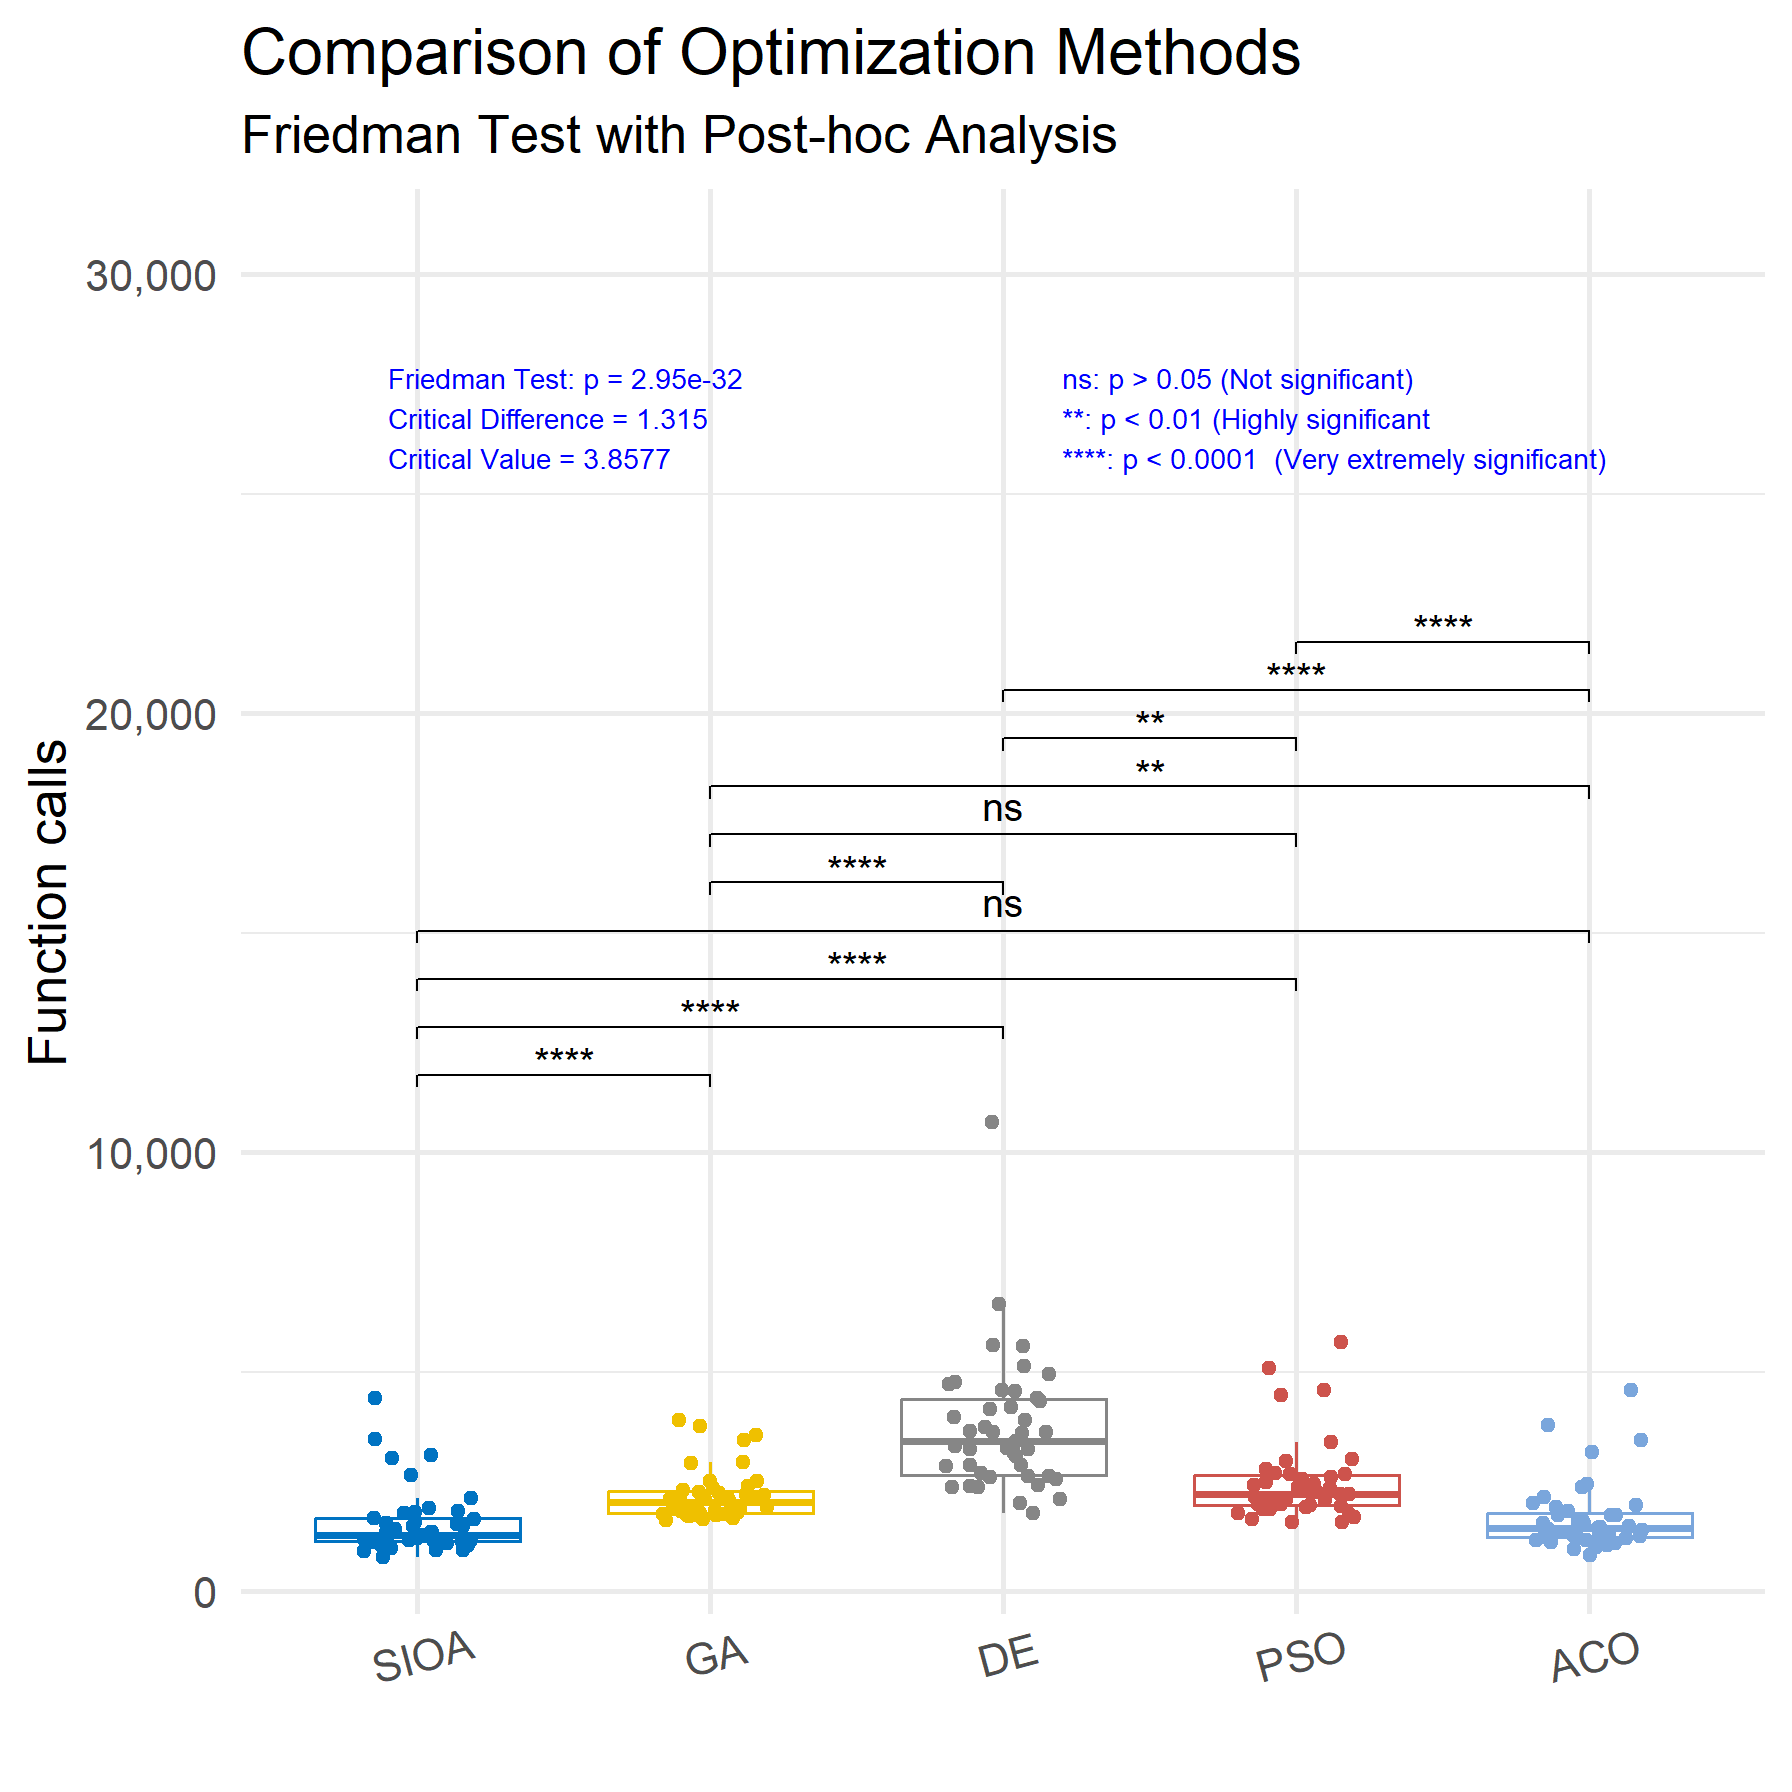
\includegraphics[scale=0.6]{friedman}
\par\end{centering}
\caption{Statistical comparison of SIOA against other methods\label{fig:SIOAvsOthers}}
\end{figure}

\begin{sidewaysfigure}[H]
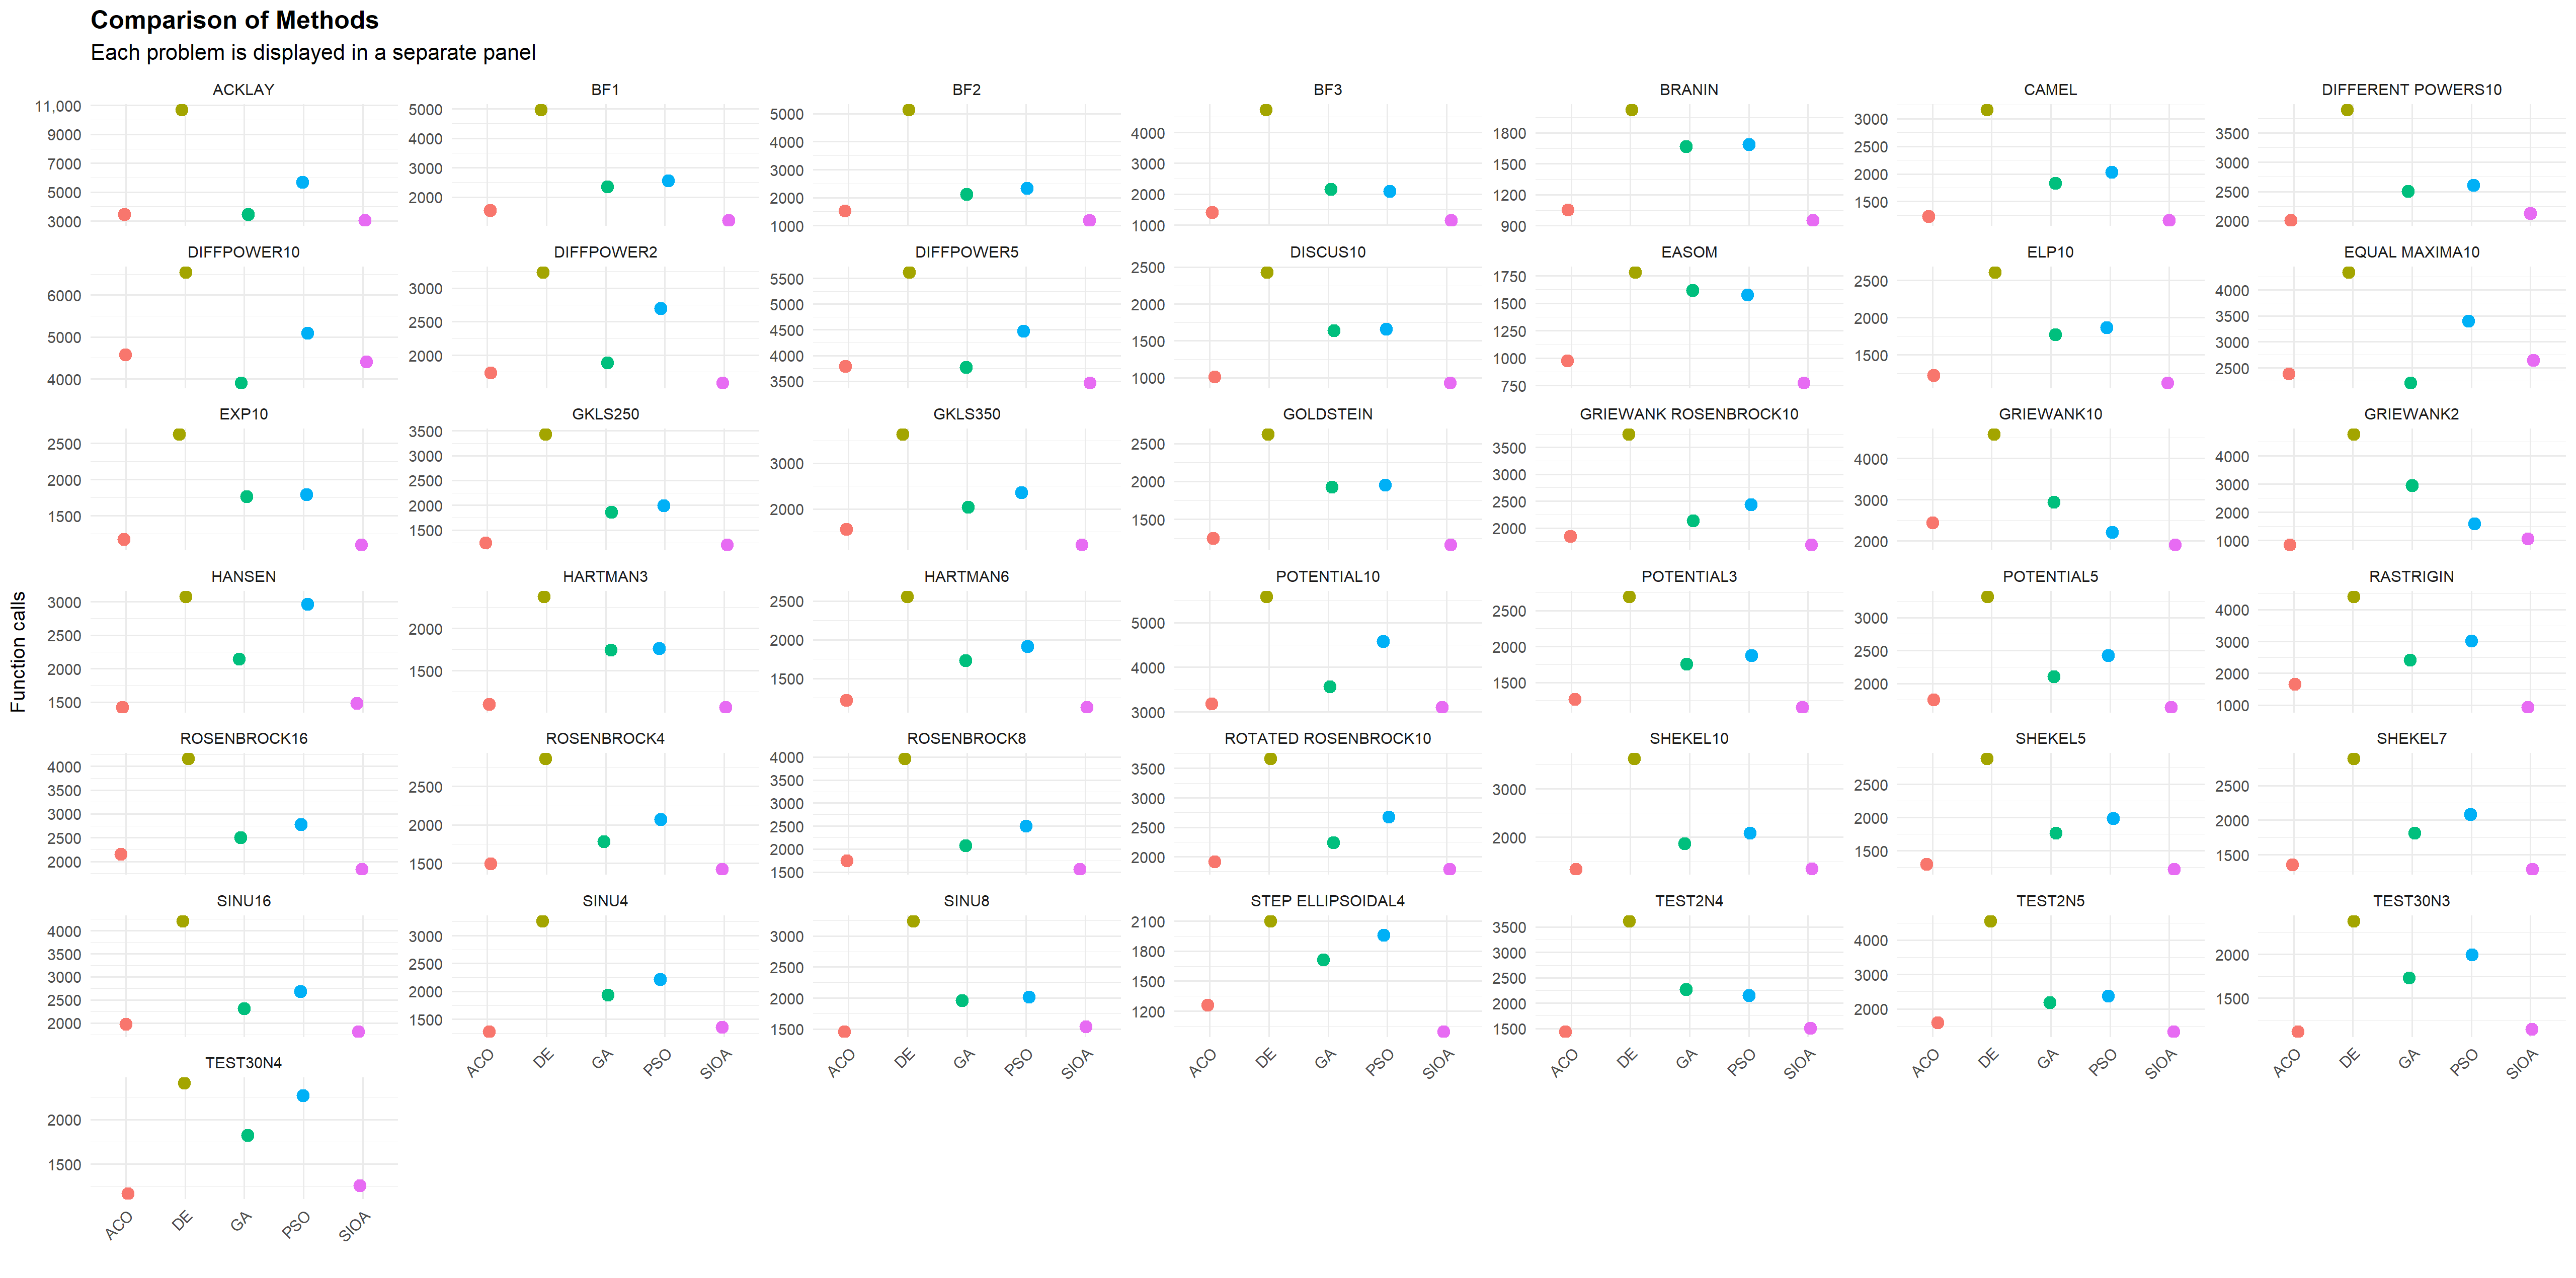
\includegraphics[scale=0.5]{table}

\caption{Performance of all methods on each problem\label{fig:performanceAllMethods}}
\end{sidewaysfigure}

The analysis of the results (Friedman test \citep{key-200}) presented
in figure {[}friedman.png{]} and table {[}table.png{]} shows the performance
comparison of the proposed SIOA optimization method against other
established techniques. The values of the critical parameter p, which
indicate the levels of statistical significance, reveal that SIOA
demonstrates a very extremely significant superiority over GA, DE,
and PSO, with p-values lower than 0.0001. In contrast, the comparison
between SIOA and ACO did not show a statistically significant difference,
as the p-value is greater than 0.05, indicating that the two methods
exhibit a similar level of performance according to this statistical
evaluation.

\subsection{Experiments with advanced methods and real-world problems\textbf{
\label{subsec:advanced=00039Cethods}} }

Subsequently, SIOA was tested against more sophisticated algorithms
on complex, large-scale problems derived from realistic application
domains, aiming to evaluate its performance under increased complexity,
constraint handling, and uncertainty.

{\tiny{}
\begin{table}[H]
{\footnotesize\caption{Real world problems CEC2011.\label{tab:realProblems}}
}{\footnotesize\par}
\centering{}{\tiny{}%
\begin{tabular}{|c|c|c|c|}
\hline 
{\tiny\textbf{PROBLEM}} & {\tiny\textbf{FORMULA}} & {\tiny\textbf{Dim}} & {\tiny\textbf{BOUNDS}}\tabularnewline
\hline 
\hline 
\begin{cellvarwidth}[t]
\centering
{\tiny\textbf{Parameter}}{\tiny\par}

{\tiny\textbf{Estimation for}}{\tiny\par}

{\tiny\textbf{Frequency-Modulated}}{\tiny\par}

{\tiny\textbf{Sound Waves}}
\end{cellvarwidth} & \begin{cellvarwidth}[t]
\centering
{\tiny$\min_{x\in[-6.4,6.35]^{6}}\;f(x)=\frac{1}{N}\sum_{n=1}^{N}\left|y(n;x)-y_{\text{target}}(n)\right|^{2}$}{\tiny\par}

{\tiny$y(n;x)=x_{0}\sin\left(x_{1}n+x_{2}\sin(x_{3}n+x_{4}\sin(x_{5}n))\right)$}
\end{cellvarwidth} & {\tiny 6} & {\tiny$x_{i}\in[-6.4,6.35]$}\tabularnewline
\hline 
\begin{cellvarwidth}[t]
\centering
{\tiny\textbf{Lennard-Jones}}{\tiny\par}

{\tiny\textbf{Potential}}
\end{cellvarwidth} & {\tiny$\min_{x\in\mathbb{R}^{3N-6}}\;f(x)=4\sum_{i=1}^{N-1}\sum_{j=i+1}^{N}\left[\left(\frac{1}{r_{ij}}\right)^{12}-\left(\frac{1}{r_{ij}}\right)^{6}\right]$} & {\tiny 30} & \begin{cellvarwidth}[t]
\centering
{\tiny$x_{0}\in(0,0,0)$}{\tiny\par}

{\tiny$x_{1},x_{2}\in[0,4]$}{\tiny\par}

{\tiny$x_{3}\in[0,\pi]$}{\tiny\par}

{\tiny$x_{3k-3}$}{\tiny\par}

{\tiny$x_{3k-2}$}{\tiny\par}

{\tiny$x_{i}\in[-b_{k},+b_{k}]$}
\end{cellvarwidth}\tabularnewline
\hline 
\begin{cellvarwidth}[t]
\centering
{\tiny\textbf{Bifunctional}}{\tiny\par}

{\tiny\textbf{Catalyst}}{\tiny\par}

{\tiny\textbf{Blend}}{\tiny\par}

{\tiny\textbf{Optimal}}{\tiny\par}

{\tiny\textbf{Control}}
\end{cellvarwidth} & \begin{cellvarwidth}[t]
\centering
{\tiny$\frac{dx_{1}}{dt}=-k_{1}x_{1}$, $\frac{dx_{2}}{dt}=k_{1}x_{1}-k_{2}x_{2}+k_{3}x_{2}+k_{4}x_{3}$,}{\tiny\par}

{\tiny$\frac{dx_{3}}{dt}=k_{2}x_{2}$, $\frac{dx_{4}}{dt}=-k_{4}x_{4}+k_{5}x_{5}$,}{\tiny\par}

{\tiny$\frac{dx_{5}}{dt}=-k_{3}x_{2}+k_{6}x_{4}-k_{5}x_{5}+k_{7}x_{6}+k_{8}x_{7}+k_{9}x_{5}+k_{10}x_{7}$}{\tiny\par}

{\tiny$\frac{dx_{6}}{dt}=k_{8}x_{5}-k_{7}x_{6}$, $\frac{dx_{7}}{dt}=k_{9}x_{5}-k_{10}x_{7}$}{\tiny\par}

{\tiny$k_{i}(u)=c_{i1}+c_{i2}u+c_{i3}u^{2}+c_{i4}u^{3}$}
\end{cellvarwidth} & {\tiny 1} & {\tiny$u\in[0.6,0.9]$}\tabularnewline
\hline 
\begin{cellvarwidth}[t]
\centering
{\tiny\textbf{Optimal}}{\tiny\par}

{\tiny\textbf{Control of a}}{\tiny\par}

{\tiny\textbf{Non-Linear}}{\tiny\par}

{\tiny\textbf{Stirred}}{\tiny\par}

{\tiny\textbf{Tank Reactor}}
\end{cellvarwidth} & \begin{cellvarwidth}[t]
\centering
{\tiny$J(u)=\int_{0}^{0.72}\left[x_{1}(t)^{2}+x_{2}(t)^{2}+0.1u^{2}\right]dt$}{\tiny\par}

{\tiny$\frac{dx_{1}}{dt}=-2x_{1}+x_{2}+1.25u+0.5\exp\left(\frac{x_{1}}{x_{1}+2}\right)$}{\tiny\par}

{\tiny$\frac{dx_{2}}{dt}=-x_{2}+0.5\exp\left(\frac{x_{1}}{x_{1}+2}\right)$}{\tiny\par}

{\tiny$x_{1}(0)=0.9,\quad x_{2}(0)=0.09$, $t\in[0,0.72]$}
\end{cellvarwidth} & {\tiny 1} & {\tiny$u\in[0,5]$}\tabularnewline
\hline 
\begin{cellvarwidth}[t]
\centering
{\tiny\textbf{Tersoff}}{\tiny\par}

{\tiny\textbf{Potential}}{\tiny\par}

{\tiny\textbf{for model Si (B)}}
\end{cellvarwidth} & \begin{cellvarwidth}[t]
\centering
{\tiny$\min_{\mathbf{x}\in\Omega}f(\mathbf{x})=\sum_{i=1}^{N}E(\mathbf{x}_{i})$}{\tiny\par}

{\tiny$E(\mathbf{x}_{i})=\frac{1}{2}\sum_{j\neq i}f_{c}(r_{ij})\left[V_{R}(r_{ij})-B_{ij}V_{A}(r_{ij})\right]$}{\tiny\par}

{\tiny where $r_{ij}=\|\mathbf{x}_{i}-\mathbf{x}_{j}\|$, $V_{R}(r)=A\exp(-\lambda_{1}r)$}{\tiny\par}

{\tiny$V_{A}(r)=B\exp(-\lambda_{2}r)$}{\tiny\par}

{\tiny$f_{c}(r)$: cutoff function with $f_{c}(r)$: angle parameter}
\end{cellvarwidth} & {\tiny 30} & \begin{cellvarwidth}[t]
\centering
{\tiny$x_{1}\in[0,4]$}{\tiny\par}

{\tiny$x_{2}\in[0,4]$}{\tiny\par}

{\tiny$x_{3}\in[0,\pi]$}{\tiny\par}

{\tiny$x_{i}\in\left[\frac{4(i-3)}{4},\ 4\right]$}
\end{cellvarwidth}\tabularnewline
\hline 
\begin{cellvarwidth}[t]
\centering
{\tiny\textbf{Tersoff}}{\tiny\par}

{\tiny\textbf{Potential}}{\tiny\par}

{\tiny\textbf{for model Si (C)}}
\end{cellvarwidth} & \begin{cellvarwidth}[t]
\centering
{\tiny$\min_{\mathbf{x}}\;V(\mathbf{x})=\sum_{i=1}^{N}\sum_{j>i}^{N}f_{C}(r_{ij})\left[a_{ij}f_{R}(r_{ij})+b_{ij}f_{A}(r_{ij})\right]$}{\tiny\par}

{\tiny$f_{C}(r)=\begin{cases}
1, & r<R-D\\
\frac{1}{2}+\frac{1}{2}\cos\left(\frac{\pi(r-R+D)}{2D}\right), & |r-R|\leq D\\
0, & r>R+D
\end{cases}$}{\tiny\par}

{\tiny$f_{R}(r)=A\exp(-\lambda_{1}r)$}{\tiny\par}

{\tiny$f_{A}(r)=-B\exp(-\lambda_{2}r)$}{\tiny\par}

{\tiny$b_{ij}=\left[1+(\beta^{n})\zeta_{ij}^{n}\right]^{-1/(2n)}$}{\tiny\par}

{\tiny$\sum_{k\neq i,j}f_{C}(r_{ik})g(\theta_{ijk})\exp\left[\lambda_{3}^{3}(r_{ij}-r_{ik})^{3}\right]$}
\end{cellvarwidth} & {\tiny 30} & \begin{cellvarwidth}[t]
\centering
{\tiny$x_{1}\in[0,4]$}{\tiny\par}

{\tiny$x_{2}\in[0,4]$}{\tiny\par}

{\tiny$x_{3}\in[0,\pi]$}{\tiny\par}

{\tiny$x_{i}\in\left[\frac{4(i-3)}{4},\ 4\right]$}
\end{cellvarwidth}\tabularnewline
\hline 
\begin{cellvarwidth}[t]
\centering
{\tiny\textbf{Spread}}{\tiny\par}

{\tiny\textbf{Spectrum Radar}}{\tiny\par}

{\tiny\textbf{Polly phase}}{\tiny\par}

{\tiny\textbf{Code Design}}
\end{cellvarwidth} & \begin{cellvarwidth}[t]
\centering
{\tiny$\min_{x\in X}\;f(x)=\max\left\{ |\varphi_{1}(x)|,|\varphi_{2}(x)|,\ldots,|\varphi_{m}(x)|\right\} $}{\tiny\par}

{\tiny$X=\{x\in\mathbb{R}^{n}\mid0\leq x_{j}\leq2\pi,\;j=1,\ldots,n\}m=2n-1$}{\tiny\par}

{\tiny$\varphi_{j}(x)=\begin{cases}
{\displaystyle \sum_{k=1}^{n-j}\cos(x_{k}-x_{k+j})} & \text{for }j=1,\ldots,n-1\\
{\displaystyle n} & \text{for }j=n\\
{\displaystyle \varphi_{2n-j}(x)} & \text{for }j=n+1,\ldots,2n-1
\end{cases}$}{\tiny\par}

{\tiny$\varphi_{j}(x)=\sum_{k=1}^{n-j}\cos(x_{k}-x_{k+j}),\quad j=1,\ldots,n-1$}{\tiny\par}

{\tiny$\varphi_{n}(x)=n$, $\varphi_{n+\ell}(x)=\varphi_{n-\ell}(x),\quad\ell=1,\ldots,n-1$}
\end{cellvarwidth} & {\tiny 20} & {\tiny$x_{j}\in[0,2\pi]$}\tabularnewline
\hline 
\begin{cellvarwidth}[t]
\centering
{\tiny\textbf{Transmission}}{\tiny\par}

{\tiny\textbf{Network}}{\tiny\par}

{\tiny\textbf{Expansion}}{\tiny\par}

{\tiny\textbf{Planning}}
\end{cellvarwidth} & \begin{cellvarwidth}[t]
\centering
{\tiny$\min\sum_{l\in\Omega}c_{l}n_{l}+W_{1}\sum_{l\in OL}|f_{l}-\bar{f}_{l}|+W_{2}\sum_{l\in\Omega}\max(0,n_{l}-\bar{n}_{l})$}{\tiny\par}

{\tiny$Sf=g-d$}{\tiny\par}

{\tiny$f_{l}=\gamma_{l}n_{l}\Delta\theta_{l},\quad\forall l\in\Omega$}{\tiny\par}

{\tiny$|f_{l}|\leq\bar{f}_{l}n_{l},\quad\forall l\in\Omega$}{\tiny\par}

{\tiny$0\leq n_{l}\leq\bar{n}_{l},\quad n_{l}\in\mathbb{Z},\quad\forall l\in\Omega$}
\end{cellvarwidth} & {\tiny 7} & \begin{cellvarwidth}[t]
\centering
{\tiny$0\leq n_{i}\leq\bar{n}_{l}$}{\tiny\par}

{\tiny$n_{i}\in\mathbb{Z}$}
\end{cellvarwidth}\tabularnewline
\hline 
\begin{cellvarwidth}[t]
\centering
{\tiny\textbf{Electricity}}{\tiny\par}

{\tiny\textbf{Transmission}}{\tiny\par}

{\tiny\textbf{Pricing}}
\end{cellvarwidth} & \begin{cellvarwidth}[t]
\centering
{\tiny$\min_{x}\;\;f(x)=\sum_{i=1}^{N_{g}}\left(\frac{C_{i}^{gen}}{P_{i}^{gen}}-R_{i}^{gen}\right)^{2}+\sum_{j=1}^{N_{d}}\left(\frac{C_{j}^{load}}{P_{j}^{load}}-R_{j}^{load}\right)^{2}$}{\tiny\par}

{\tiny$\sum_{j}GD_{i,j}+\sum_{j}BT_{i,j}=P_{i}^{gen},\quad\forall i$}{\tiny\par}

{\tiny$\sum_{i}GD_{i,j}+\sum_{i}BT_{i,j}=P_{j}^{load},\quad\forall j$}{\tiny\par}

{\tiny$GD_{i,j}^{max}=\min(P_{i}^{gen}-BT_{i,j},\;P_{j}^{load}-BT_{i,j})$}
\end{cellvarwidth} & {\tiny 126} & {\tiny$GD_{i,j}\in[0,GD_{i,j}^{max}]$}\tabularnewline
\hline 
\begin{cellvarwidth}[t]
\centering
{\tiny\textbf{Circular}}{\tiny\par}

{\tiny\textbf{Antenna}}{\tiny\par}

{\tiny\textbf{Array}}{\tiny\par}

{\tiny\textbf{Design}}
\end{cellvarwidth} & \begin{cellvarwidth}[t]
\centering
{\tiny$\min_{r_{1},\ldots,r_{6},\,\varphi_{1},\ldots,\varphi_{6}}\quad f(\mathbf{x})=\max_{\theta\in\Omega}AF(\mathbf{x},\theta)$}{\tiny\par}

{\tiny$AF(\mathbf{x},\theta)=\left|\sum_{k=1}^{6}\exp\left(j\left[2\pi r_{k}\cos(\theta-\theta_{k})+\varphi_{k}\frac{\pi}{180}\right]\right)\right|$}
\end{cellvarwidth} & {\tiny 12} & \begin{cellvarwidth}[t]
\centering
{\tiny$r_{k}\in[0.2,1]$}{\tiny\par}

{\tiny$\varphi_{k}\in[-180,180]$}
\end{cellvarwidth}\tabularnewline
\hline 
\begin{cellvarwidth}[t]
\centering
{\tiny\textbf{Dynamic}}{\tiny\par}

{\tiny\textbf{Economic}}{\tiny\par}

{\tiny\textbf{Dispatch 1}}
\end{cellvarwidth} & \begin{cellvarwidth}[t]
\centering
{\tiny$\min_{\mathbf{P}}\quad f(\mathbf{P})=\sum_{t=1}^{24}\sum_{i=1}^{5}\left(a_{i}P_{i,t}^{2}+b_{i}P_{i,t}+c_{i}\right)$}{\tiny\par}

{\tiny$P_{i}^{\min}\leq P_{i,t}\leq P_{i}^{\max},\quad\forall i=1,\ldots,5,\;t=1,\ldots,24$}{\tiny\par}

{\tiny$\sum_{i=1}^{5}P_{i,t}=D_{t},\quad\forall t=1,\ldots,24$}{\tiny\par}

{\tiny$P_{\min}=[10,20,30,40,50]$}{\tiny\par}

{\tiny$P_{\max}=[75,125,175,250,300]$}
\end{cellvarwidth} & {\tiny 120} & {\tiny$P_{i}^{\min}\leq P_{i,t}\leq P_{i}^{\max}$}\tabularnewline
\hline 
\begin{cellvarwidth}[t]
\centering
{\tiny\textbf{Dynamic}}{\tiny\par}

{\tiny\textbf{Economic}}{\tiny\par}

{\tiny\textbf{Dispatch 2}}
\end{cellvarwidth} & \begin{cellvarwidth}[t]
\centering
{\tiny$\min_{\mathbf{P}}\quad f(\mathbf{P})=\sum_{t=1}^{24}\sum_{i=1}^{9}\left(a_{i}P_{i,t}^{2}+b_{i}P_{i,t}+c_{i}\right)$}{\tiny\par}

{\tiny$P_{i}^{\min}\leq P_{i,t}\leq P_{i}^{\max},\quad\forall i=1,\ldots,5,\;t=1,\ldots,24$}{\tiny\par}

{\tiny$\sum_{i=1}^{5}P_{i,t}=D_{t},\quad\forall t=1,\ldots,24$}{\tiny\par}

{\tiny$P_{\min}=[150,135,73,60,73,57,20,47,20]$}{\tiny\par}

{\tiny$P_{\max}=[470,460,340,300,243,160,130,120,80]$}
\end{cellvarwidth} & {\tiny 216} & {\tiny$P_{i}^{\min}\leq P_{i,t}\leq P_{i}^{\max}$}\tabularnewline
\hline 
\begin{cellvarwidth}[t]
\centering
{\tiny\textbf{Static}}{\tiny\par}

{\tiny\textbf{Economic}}{\tiny\par}

{\tiny\textbf{Load}}{\tiny\par}

{\tiny\textbf{Dispatch}}{\tiny\par}

{\tiny\textbf{(1,2,3,4,5)}}
\end{cellvarwidth} & \begin{cellvarwidth}[t]
\centering
{\tiny$\min_{P_{1},\ldots,P_{N_{G}}}F=\sum_{i=1}^{N_{G}}f_{i}(P_{i})$}{\tiny\par}

{\tiny$f_{i}(P_{i})=a_{i}P_{i}^{2}+b_{i}P_{i}+c_{i},\quad i=1,2,\ldots,N_{G}$}{\tiny\par}

{\tiny$f_{i}(P_{i})=a_{i}P_{i}^{2}+b_{i}P_{i}+c_{i}+|e_{i}\sin(f_{i}(P_{i}^{\min}-P_{i}))|$}{\tiny\par}

{\tiny$P_{i}^{\min}\leq P_{i}\leq P_{i}^{\max},\quad i=1,2,\ldots,N_{G}$}{\tiny\par}

{\tiny$\sum_{i=1}^{N_{G}}P_{i}=P_{D}+P_{L}$}{\tiny\par}

{\tiny$P_{L}=\sum_{i=1}^{N_{G}}\sum_{j=1}^{N_{G}}P_{i}B_{ij}P_{j}+\sum_{i=1}^{N_{G}}B_{0i}P_{i}+B_{00}$}{\tiny\par}

{\tiny$P_{i}-P_{i}^{0}\leq UR_{i}\quad P_{i}^{0}-P_{i}\leq DR_{i}$}
\end{cellvarwidth} & \begin{cellvarwidth}[t]
\centering
{\tiny 6}{\tiny\par}

{\tiny 13}{\tiny\par}

{\tiny 15}{\tiny\par}

{\tiny 40}{\tiny\par}

{\tiny 140}
\end{cellvarwidth} & \begin{cellvarwidth}[t]
\centering
{\tiny See}{\tiny\par}

{\tiny Technical}{\tiny\par}

{\tiny Report}{\tiny\par}

{\tiny of}{\tiny\par}

{\tiny CEC2011}
\end{cellvarwidth}\tabularnewline
\hline 
\end{tabular}}{\tiny\par}
\end{table}
}{\tiny\par}

The results shown in Table \ref{tab:betterAlgorithms} were obtained
using the parameter settings defined in Table \ref{tab:settings}.
The termination criterion was set to 150,000 function evaluations,
ensuring a uniform computational budget across all test cases. No
local optimization procedures were applied during the runs, meaning
that the reported outcomes reflect solely the global search capabilities
of the algorithm without any refinement from local search techniques.
This setup allows for an unbiased assessment of the method’s performance
under purely global exploration conditions.

{\tiny{}
\begin{sidewaystable}[H]
\caption{Algorithms’ Comparison Based on Best and Mean after 1.5e+5 FEs\label{tab:betterAlgorithms}}

\begin{centering}
\begin{tabular}{|c|c|c|c|c|c|c|c|c|c|c|c|c|c|c|c|}
\hline 
150000 Fes & \multicolumn{3}{c|}{CLPSO} & \multicolumn{3}{c|}{SaDE} & \multicolumn{3}{c|}{jDE} & \multicolumn{3}{c|}{CMA-ES} & \multicolumn{3}{c|}{SIOA}\tabularnewline
\hline 
\hline 
{\tiny\textbf{Problem}} & {\tiny\textbf{best}} & {\tiny\textbf{mean}} & {\tiny\textbf{st}} & {\tiny\textbf{best}} & {\tiny\textbf{mean}} & {\tiny\textbf{st}} & {\tiny\textbf{best}} & {\tiny\textbf{mean}} & {\tiny\textbf{st}} & {\tiny\textbf{best}} & {\tiny\textbf{mean}} & {\tiny\textbf{st}} & {\tiny\textbf{best}} & {\tiny\textbf{mean}} & {\tiny\textbf{st}}\tabularnewline
\hline 
\begin{cellvarwidth}[t]
\centering
{\tiny\textbf{Parameter}}{\tiny\par}

{\tiny\textbf{Estimation for}}{\tiny\par}

{\tiny\textbf{Frequency-Modulated}}{\tiny\par}

{\tiny\textbf{Sound Waves}}
\end{cellvarwidth} & {\tiny 0.1314837477} & {\tiny 0.2124981688} & {\tiny 0.030223102} & {\tiny 0.1899428536} & {\tiny 0.2025566839} & {\tiny 0.009271896} & {\tiny 0.116157541} & {\tiny 0.146008756} & {\tiny 0.035009569} & {\tiny 0.18160915970} & {\tiny 0.256863966} & {\tiny 0.044727545} & {\tiny 0.20618586} & {\tiny 0.259930863} & {\tiny 0.023021357}\tabularnewline
\hline 
\begin{cellvarwidth}[t]
\centering
{\tiny\textbf{Lennard-Jones}}{\tiny\par}

{\tiny\textbf{Potential}}
\end{cellvarwidth} & {\tiny -13.43649135} & {\tiny -10.25073403} & {\tiny 1.02903617} & {\tiny -24.86870825} & {\tiny -22.6693403} & {\tiny 1.127265561} & {\tiny -29.98126575} & {\tiny -27.49258505} & {\tiny 1.235083397} & {\tiny -28.42253189} & {\tiny -25.78783328} & {\tiny 2.27119571} & {\tiny -28.51132554} & {\tiny -24.14612379} & {\tiny 2.489334694}\tabularnewline
\hline 
\begin{cellvarwidth}[t]
\centering
{\tiny\textbf{Bifunctional}}{\tiny\par}

{\tiny\textbf{Catalyst Blend}}{\tiny\par}

{\tiny\textbf{Optimal Control}}
\end{cellvarwidth} & {\tiny -0.000286591} & {\tiny -0.000286591} & {\tiny 1.157726295e-16} & {\tiny -0.000286591} & {\tiny -0.000286591} & {\tiny 5.513684428e-20} & {\tiny -0.000286591} & {\tiny -0.000286591} & {\tiny 5.513684428e-20} & {\tiny -0.000286591} & {\tiny -0.000286591} & {\tiny 5.513684428e-20} & {\tiny -0.000286591} & {\tiny -0.000286591} & {\tiny 9.177681044e-11}\tabularnewline
\hline 
\begin{cellvarwidth}[t]
\centering
{\tiny\textbf{Optimal Control of a}}{\tiny\par}

{\tiny\textbf{Non-Linear Stirred}}{\tiny\par}

{\tiny\textbf{Tank Reactor}}
\end{cellvarwidth} & {\tiny 0.3903767228} & {\tiny 0.3903767228} & {\tiny 0.00} & {\tiny 0.3903767228} & {\tiny 0.3903767228} & {\tiny 0.00} & {\tiny 0.390376723} & {\tiny 0.390376723} & {\tiny 0} & {\tiny 0.3903767228} & {\tiny 0.390376723} & {\tiny 0} & {\tiny 0.390376723} & {\tiny 0.390376723} & {\tiny 0}\tabularnewline
\hline 
\begin{cellvarwidth}[t]
\centering
{\tiny\textbf{Tersoff Potential}}{\tiny\par}

{\tiny\textbf{for model Si (B)}}
\end{cellvarwidth} & {\tiny -28.23544117} & {\tiny -26.18834522} & {\tiny 1.05654251} & {\tiny -3.107773136} & {\tiny 25.4711091} & {\tiny 16.7202543} & {\tiny -13.51157064} & {\tiny -3.983690794} & {\tiny 6.666047747} & {\tiny -29.26244222} & {\tiny -27.5889735} & {\tiny 1.040646284} & {\tiny -28.63594613} & {\tiny -27.11517851} & {\tiny 1.084722973}\tabularnewline
\hline 
\begin{cellvarwidth}[t]
\centering
{\tiny\textbf{Tersoff Potential}}{\tiny\par}

{\tiny\textbf{for model Si (C)}}
\end{cellvarwidth} & {\tiny -30.85200257} & {\tiny -28.87349048} & {\tiny 0.988024149} & {\tiny -11.60719468} & {\tiny 22.08963599} & {\tiny 18.5809093} & {\tiny -18.76214649} & {\tiny -8.506037168} & {\tiny 5.543190141} & {\tiny -33.19699356} & {\tiny -31.79270914} & {\tiny 0.828194234} & {\tiny -33.50417851} & {\tiny -31.0138182} & {\tiny 1.420690601}\tabularnewline
\hline 
\begin{cellvarwidth}[t]
\centering
{\tiny\textbf{Spread Spectrum}}{\tiny\par}

{\tiny\textbf{Radar Polly phase}}{\tiny\par}

{\tiny\textbf{Code Design}}
\end{cellvarwidth} & {\tiny 1.085334991} & {\tiny 1.343956153} & {\tiny 0.148708837} & {\tiny 1.536501579} & {\tiny 2.150881715} & {\tiny 0.198607499} & {\tiny 1.525870558} & {\tiny 1.812042166} & {\tiny 0.171213339} & {\tiny 0.01484822722} & {\tiny 0.171988666} & {\tiny 0.137892008} & {\tiny 0.607180067} & {\tiny 1.023498006} & {\tiny 0.228610721}\tabularnewline
\hline 
\begin{cellvarwidth}[t]
\centering
{\tiny\textbf{Transmission Network}}{\tiny\par}

{\tiny\textbf{Expansion Planning}}
\end{cellvarwidth} & {\tiny 250.00} & {\tiny 250.00} & {\tiny 0.00} & {\tiny 250.00} & {\tiny 250.00} & {\tiny 0.00} & {\tiny 250.00} & {\tiny 250.00} & {\tiny 0.00} & {\tiny 250.00} & {\tiny 250.00} & {\tiny 0.00} & {\tiny 250.00} & {\tiny 250.00} & {\tiny 0}\tabularnewline
\hline 
\begin{cellvarwidth}[t]
\centering
{\tiny\textbf{Electricity}}{\tiny\par}

{\tiny\textbf{Transmission Pricing}}
\end{cellvarwidth} & {\tiny 13,775,010.10} & {\tiny 13,775,395.07} & {\tiny 222.9723613} & {\tiny 23,481,009.86} & {\tiny 30,034,934.81} & {\tiny 3,264,767.4} & {\tiny 13,774,627.84} & {\tiny 14,020,953.78} & {\tiny 276,142.5345} & {\tiny 13,775,841.77} & {\tiny 13,787,550.18} & {\tiny 6136.744382} & {\tiny 13,774,551.1} & {\tiny 13,775,341.62} & {\tiny 372.2433548}\tabularnewline
\hline 
\begin{cellvarwidth}[t]
\centering
{\tiny\textbf{Circular Antenna}}{\tiny\par}

{\tiny\textbf{Array Design}}
\end{cellvarwidth} & {\tiny 0.006933401045} & {\tiny 0.05181551798} & {\tiny 0.070674314} & {\tiny 0.02142329927} & {\tiny 0.03892428051} & {\tiny 0.008183211} & {\tiny 0.006820072} & {\tiny 0.017657998} & {\tiny 0.022383475} & {\tiny 0.007204797576} & {\tiny 0.008635655364} & {\tiny 0.000917821} & {\tiny 0.007425975} & {\tiny 0.024989563} & {\tiny 0.044360116}\tabularnewline
\hline 
\begin{cellvarwidth}[t]
\centering
{\tiny\textbf{Dynamic Economic}}{\tiny\par}

{\tiny\textbf{Dispatch 1}}
\end{cellvarwidth} & {\tiny 428,607,927.60} & {\tiny 435,250,914.50} & {\tiny 2,973,190.125} & {\tiny 968,042,312.10} & {\tiny 1,034,679,775.00} & {\tiny 25667290.12} & {\tiny 968,042,312.1} & {\tiny 1,034,393,036} & {\tiny 25,445,935.78} & {\tiny 88,285.60} & {\tiny 102,776.71} & {\tiny 6688.08697} & {\tiny 921,434,356.7} & {\tiny 984,699,299.8} & {\tiny 23,606,727.92}\tabularnewline
\hline 
\begin{cellvarwidth}[t]
\centering
{\tiny\textbf{Dynamic Economic}}{\tiny\par}

{\tiny\textbf{Dispatch 2}}
\end{cellvarwidth} & {\tiny 33,031,590.31} & {\tiny 53,906,147.38} & {\tiny 8,492,239.111} & {\tiny 845,287,898.30} & {\tiny 913,715,793.20} & {\tiny 3,0667,287.54} & {\tiny 340,091,475.3} & {\tiny 397,471,715.1} & {\tiny 37,259,947.14} & {\tiny 502,699.42} & {\tiny 477,720.15} & {\tiny 193,951.4891} & {\tiny 768,167,675.2} & {\tiny 768,167,675.2} & {\tiny 768,167,675.2}\tabularnewline
\hline 
\begin{cellvarwidth}[t]
\centering
{\tiny\textbf{StaticEconomic}}{\tiny\par}

{\tiny\textbf{Load Dispatch 1}}
\end{cellvarwidth} & {\tiny 6554.67} & {\tiny 7668.33} & {\tiny 1245.137667} & {\tiny 16,877.92} & {\tiny 101,588.39} & {\tiny 81105.92078} & {\tiny 6163.749006} & {\tiny 6778.527028} & {\tiny 3004.59066} & {\tiny 6657.61} & {\tiny 415,917.46} & {\tiny 688,544.4983} & {\tiny 6538.455462} & {\tiny 877,097.0217} & {\tiny 847,631.4535}\tabularnewline
\hline 
\begin{cellvarwidth}[t]
\centering
{\tiny\textbf{Static Economic}}{\tiny\par}

{\tiny\textbf{Load Dispatch 2}}
\end{cellvarwidth} & {\tiny 19,030.36} & {\tiny 20,699.00} & {\tiny 2922.047235} & {\tiny 2,600,565.21} & {\tiny 9,329,466.81} & {\tiny 4,019,053.284} & {\tiny 1,161,578.904} & {\tiny 3,671,587.605} & {\tiny 1,542,286.275} & {\tiny 763,001.22} & {\tiny 1,425,815.44} & {\tiny 377,126.8219} & {\tiny 24,026.88184} & {\tiny 1,478,534.024} & {\tiny 1,063,608.234}\tabularnewline
\hline 
\begin{cellvarwidth}[t]
\centering
{\tiny\textbf{Static Economic}}{\tiny\par}

{\tiny\textbf{Load Dispatch 3}}
\end{cellvarwidth} & {\tiny 470,192,288.30} & {\tiny 470,294,703.20} & {\tiny 57822.41621} & {\tiny 478,069,615.30} & {\tiny 541,898,763.00} & {\tiny 20,128,777.18} & {\tiny 471,058,115.8} & {\tiny 471,963,142.3} & {\tiny 529,633.389} & {\tiny 470,023,232.30} & {\tiny 470,023,232.30} & {\tiny 1.848771369e-07} & {\tiny 470,825,156.9} & {\tiny 472,256,736.5} & {\tiny 608,886.262}\tabularnewline
\hline 
\begin{cellvarwidth}[t]
\centering
{\tiny\textbf{Static Economic}}{\tiny\par}

{\tiny\textbf{Load Dispatch 4}}
\end{cellvarwidth} & {\tiny 884,980.56} & {\tiny 1,423,887.36} & {\tiny 285,794.4518} & {\tiny 14,170,362.58} & {\tiny 106,749,078.50} & {\tiny 73,147,979.72} & {\tiny 6,482,592.714} & {\tiny 17,527,314.24} & {\tiny 53,06,489.46} & {\tiny 476,053.52} & {\tiny 2,925,852.94} & {\tiny 12,68,161.817} & {\tiny 70,686.26733} & {\tiny 580,122.834} & {\tiny 340,707.3484}\tabularnewline
\hline 
\begin{cellvarwidth}[t]
\centering
{\tiny\textbf{Static Economic}}{\tiny\par}

{\tiny\textbf{Load Dispatch 15}}
\end{cellvarwidth} & {\tiny 8,105,947,615} & {\tiny 8,110,924,071.00} & {\tiny 4,422,895.726} & {\tiny 1.312720405e+10} & {\tiny 13,543,754,650.00} & {\tiny 213,865,059.7} & {\tiny 8,453,090,778} & {\tiny 8,459,337,082} & {\tiny 2874,979.192} & {\tiny 8,072,077,963} & {\tiny 8,084,017,791} & {\tiny 4,623,617.36} & {\tiny 8,002,077,963} & {\tiny 8,048,300,791} & {\tiny 4,365,204.42}\tabularnewline
\hline 
\end{tabular}
\par\end{centering}
\end{sidewaystable}
}
\begin{sidewaystable}[H]
\caption{Detailed Ranking of Algorithms Based on Best and Mean after 1.5e+5
FEs\label{tab:rankingBestAndMean}}

\centering{}{\footnotesize{}%
\begin{tabular}{|V{\linewidth}|c|c|c|c|c|c|c|c|c|c|}
\hline 
{\footnotesize\textbf{Problem}} & \begin{cellvarwidth}[t]
\centering
{\footnotesize\textbf{CLPSO}}{\footnotesize\par}

{\footnotesize\textbf{best}}
\end{cellvarwidth} & \begin{cellvarwidth}[t]
\centering
{\footnotesize\textbf{CLPSO}}{\footnotesize\par}

{\footnotesize\textbf{Mean}}
\end{cellvarwidth} & \begin{cellvarwidth}[t]
\centering
{\footnotesize\textbf{SaDE}}{\footnotesize\par}

{\footnotesize\textbf{best}}
\end{cellvarwidth} & \begin{cellvarwidth}[t]
\centering
{\footnotesize\textbf{SaDE}}{\footnotesize\par}

{\footnotesize\textbf{Mean}}
\end{cellvarwidth} & \begin{cellvarwidth}[t]
\centering
{\footnotesize\textbf{jDE}}{\footnotesize\par}

{\footnotesize\textbf{Best}}
\end{cellvarwidth} & \begin{cellvarwidth}[t]
\centering
{\footnotesize\textbf{jDE}}{\footnotesize\par}

{\footnotesize\textbf{Mean}}
\end{cellvarwidth} & \begin{cellvarwidth}[t]
\centering
{\footnotesize\textbf{CMA-ES}}{\footnotesize\par}

{\footnotesize\textbf{best}}
\end{cellvarwidth} & \begin{cellvarwidth}[t]
\centering
{\footnotesize\textbf{CMA-ES}}{\footnotesize\par}

{\footnotesize\textbf{Mean}}
\end{cellvarwidth} & \begin{cellvarwidth}[t]
\centering
{\footnotesize\textbf{EO}}{\footnotesize\par}

{\footnotesize\textbf{Best}}
\end{cellvarwidth} & \begin{cellvarwidth}[t]
\centering
{\footnotesize\textbf{EO}}{\footnotesize\par}

{\footnotesize\textbf{Mean}}
\end{cellvarwidth}\tabularnewline
\hline 
\hline 
{\footnotesize\textbf{Parameter Estimation for}}{\footnotesize\par}

{\footnotesize\textbf{Frequency-Modulated Sound Waves}} & 2 & 3 & 4 & 2 & 1 & 1 & 3 & 4 & 5 & 5\tabularnewline
\hline 
{\footnotesize\textbf{Lennard-Jones}}{\footnotesize\par}

{\footnotesize\textbf{Potential}} & 5 & 5 & 4 & 4 & 1 & 1 & 3 & 2 & 2 & 3\tabularnewline
\hline 
{\footnotesize\textbf{BifunctionalCatalyst Blend}}{\footnotesize\par}

{\footnotesize\textbf{Optimal Control}} & 1 & 1 & 1 & 1 & 1 & 1 & 1 & 1 & 1 & 1\tabularnewline
\hline 
{\footnotesize\textbf{Optimal Control of a}}{\footnotesize\par}

{\footnotesize\textbf{Non-Linear Stirred}}{\footnotesize\par}

{\footnotesize\textbf{Tank Reactor}} & 1 & 1 & 1 & 1 & 1 & 1 & 1 & 1 & 1 & 1\tabularnewline
\hline 
{\footnotesize\textbf{Tersoff Potential}}{\footnotesize\par}

{\footnotesize\textbf{for model Si (B)}} & 3 & 3 & 5 & 5 & 4 & 4 & 1 & 1 & 2 & 2\tabularnewline
\hline 
{\footnotesize\textbf{Tersoff Potential}}{\footnotesize\par}

{\footnotesize\textbf{for model Si (C)}} & 3 & 3 & 5 & 5 & 4 & 4 & 2 & 1 & 1 & 2\tabularnewline
\hline 
{\footnotesize\textbf{Spread Spectrum Radar}}{\footnotesize\par}

{\footnotesize\textbf{Polly phaseCode Design}} & 3 & 3 & 5 & 5 & 4 & 4 & 1 & 1 & 2 & 2\tabularnewline
\hline 
{\footnotesize\textbf{Transmission Network}}{\footnotesize\par}

{\footnotesize\textbf{Expansion Planning}} & 1 & 1 & 1 & 1 & 1 & 1 & 1 & 1 & 1 & 1\tabularnewline
\hline 
{\footnotesize\textbf{Electricity Transmission}}{\footnotesize\par}

{\footnotesize\textbf{Pricing}} & 3 & 1 & 5 & 5 & 2 & 4 & 4 & 3 & 1 & 2\tabularnewline
\hline 
{\footnotesize\textbf{Circular Antenna}}{\footnotesize\par}

{\footnotesize\textbf{Array Design}} & 2 & 5 & 5 & 4 & 1 & 2 & 3 & 1 & 4 & 3\tabularnewline
\hline 
{\footnotesize\textbf{Dynamic Economic}}{\footnotesize\par}

{\footnotesize\textbf{Dispatch 1}} & 2 & 2 & 5 & 5 & 4 & 4 & 1 & 1 & 3 & 3\tabularnewline
\hline 
{\footnotesize\textbf{Dynamic Economic}}{\footnotesize\par}

{\footnotesize\textbf{Dispatch 2}} & 2 & 2 & 5 & 5 & 3 & 3 & 1 & 1 & 4 & 4\tabularnewline
\hline 
{\footnotesize\textbf{Static Economic}}{\footnotesize\par}

{\footnotesize\textbf{Load Dispatch 1}} & 3 & 2 & 5 & 5 & 1 & 1 & 4 & 3 & 2 & 4\tabularnewline
\hline 
{\footnotesize\textbf{Static Economic}}{\footnotesize\par}

{\footnotesize\textbf{Load Dispatch 2}} & 1 & 1 & 5 & 5 & 4 & 4 & 3 & 2 & 2 & 3\tabularnewline
\hline 
{\footnotesize\textbf{Static Economic}}{\footnotesize\par}

{\footnotesize\textbf{Load Dispatch 3}} & 2 & 2 & 5 & 5 & 4 & 3 & 1 & 1 & 3 & 4\tabularnewline
\hline 
{\footnotesize\textbf{Static Economic}}{\footnotesize\par}

{\footnotesize\textbf{Load Dispatch 4}} & 3 & 2 & 5 & 5 & 4 & 4 & 2 & 3 & 1 & 1\tabularnewline
\hline 
{\footnotesize\textbf{Static Economic}}{\footnotesize\par}

{\footnotesize\textbf{Load Dispatch 5}} & 3 & 3 & 5 & 5 & 4 & 4 & 2 & 2 & 1 & 1\tabularnewline
\hline 
{\footnotesize\textbf{TOTAL}} & \textbf{40} & \textbf{40} & \textbf{71} & \textbf{68} & \textbf{44} & \textbf{46} & \textbf{34} & \textbf{29} & \textbf{36} & \textbf{42}\tabularnewline
\hline 
\end{tabular}}{\footnotesize\par}
\end{sidewaystable}
\begin{table}[H]
\caption{Comparison of Algorithms and Final Ranking\label{tab:finalRanking}}

\centering{}%
\begin{tabular}{|c|c|c|c|c|c|}
\hline 
Method & \textbf{Best} & \textbf{Mean} & \textbf{Overall} & \textbf{Average} & \textbf{Rang}\tabularnewline
\hline 
\hline 
CMA-ES & 34 & 29 & 63 & 1.75 & 1\tabularnewline
\hline 
EO & 36 & 42 & 78 & 2.16 & 2\tabularnewline
\hline 
CLPSO & 40 & 40 & 80 & 2.22 & 3\tabularnewline
\hline 
jDE & 44 & 46 & 90 & 2.5 & 4\tabularnewline
\hline 
SaDE & 71 & 68 & 139 & 3.86 & 5\tabularnewline
\hline 
\end{tabular}
\end{table}

The comparative analysis of the optimization methods, based on both
best and mean performance after 150,000 function evaluations, reveals
clear distinctions in their overall effectiveness. CMA-ES achieved
the highest ranking, excelling in both peak and consistent performance,
followed by EO and CLPSO, which demonstrated strong competitiveness.
SIOA ranked closely behind these top methods, showing notable strengths
in complex, high-dimensional, and multimodal problems, where its adaptive
sporulation and germination mechanisms effectively balanced exploration
and exploitation. In certain cases, such as the Tersoff Potential
and Static Economic Load Dispatch problems, SIOA’s results approached
those of CMA-ES, highlighting its capacity to rival advanced evolutionary
strategies. However, its slightly higher variance in some problem
instances, particularly in less multimodal landscapes, reduced its
mean performance score, preventing it from achieving the top overall
rank. Despite this, SIOA emerges as a modern and competitive algorithm
with strong potential for further improvement, especially through
integration with specialized local search schemes aimed at enhancing
stability and precision.

\subsection{Exploration and exploitation\label{subsec:exploration=000395xploitation}}

In this study, the trade-off between exploration and exploitation
is assessed using a specific set of quantitative indicators: Initial
Population Diversity ($IPD$), Final Population Diversity ($FPD$),
Average Exploration Ratio ($AER$), Median Exploration Ratio ($MER$),
and Average Balance Index ($ABI$). These metrics, although fundamentally
grounded in population diversity measurements, are designed to capture
both the temporal evolution of exploration by monitoring diversity
changes over the course of the optimization and the degree of exploitation
through the level of convergence in the final population. While these
indicators provide a structured way to examine algorithmic behavior,
further investigation employing more direct analysis tools, such as
attraction basin mapping or tracking the clustering of solutions around
local or global optima, could yield deeper insights into the search
dynamics. Such approaches are considered a promising avenue for extending
the current work.

The metrics reported in Tables \ref{tab:abi} quantify and track the
interplay between exploration and exploitation throughout the execution
of the SIOA algorithm. Their computation relies on diversity measurements
at different stages of the optimization process and on how these values
evolve over iterations.

The $IPD$ quantifies the diversity present at the very start of the
optimization and is obtained by computing the mean Euclidean distance
between all pairs of individuals in the initial population:

\begin{equation}
IPD=\frac{2}{NP(NP-1)}\sum_{i=1}^{NP-1}\sum_{j=i+1}^{NP}d(x_{i},x_{j})
\end{equation}

where $d(x_{i},x_{j})$ is the Euclidean distance between solutions
$x_{i}$and $x_{j}$end $NP$ denotes the population size.

The $FPD$ is computed using the same formulation, but applied to
the final set of solutions after the algorithm completes.

The $AER$ reflects the average level of exploration across all iterations
and is defined as:

\begin{equation}
AER=\frac{1}{G}\sum_{g=1}^{iter_{max}}\frac{IPD_{g}}{IPD_{1}}
\end{equation}

where $iter_{max}$is the total number of iterations, $IPD_{g}$represents
the diversity at iteration $g$, and $IPD_{1}$ is the initial diversity
value.

The $MER$ is the median value of the exploration ratios recorded
over all generations:

\begin{equation}
MER=\text{median}\left(\frac{IPD_{g}}{IPD_{1}}\right),\quad\text{for }g=1,\dots,iter_{max}
\end{equation}

The $ABI$ serves as a composite measure of the exploration--exploitation
balance. It is typically calculated as a weighted function of $AER$
and $FPD$ (or other exploitation-related indicators):

\begin{equation}
ABI=\frac{AER}{AER+\epsilon}\cdot\left(1-\frac{FPD}{IPD}\right)
\end{equation}

where $\epsilon$ is a small constant introduced to avoid division
by zero. An $ABI$ value close to 0.5 generally indicates a well-balanced
interplay between exploration and exploitation.

\begin{table}[H]
\caption{Balance between exploration and exploitation of the SIOA method in
each benchmark function after 1.5e+5 FEs\label{tab:abi}}

\begin{centering}
{\tiny{}%
\begin{tabular}{|c|c|c|c|c|c|c|c|c|}
\hline 
{\tiny PROBLEM} & {\tiny BEST} & {\tiny MEAN} & {\tiny SD} & {\tiny IPD} & {\tiny FDP} & {\tiny AER} & {\tiny MER} & {\tiny ABI}\tabularnewline
\hline 
\hline 
\begin{cellvarwidth}[t]
\centering
{\tiny\textbf{Parameter}}{\tiny\par}

{\tiny\textbf{Estimation for}}{\tiny\par}

{\tiny\textbf{Frequency-Modulated}}{\tiny\par}

{\tiny\textbf{Sound Waves}}
\end{cellvarwidth} & {\tiny 0.20618586} & {\tiny 0.259930863} & {\tiny 0.023021357} & {\tiny 8.5901} & {\tiny 4.16015} & {\tiny 4.16015} & {\tiny 0} & {\tiny 0.49979}\tabularnewline
\hline 
\begin{cellvarwidth}[t]
\centering
{\tiny\textbf{Lennard-Jones}}{\tiny\par}

{\tiny\textbf{Potential}}
\end{cellvarwidth} & {\tiny -28.51132554} & {\tiny -24.14612379} & {\tiny 2.489334694} & {\tiny 13.91823} & {\tiny 4.466} & {\tiny 0.00021} & {\tiny 0} & {\tiny 0.49967}\tabularnewline
\hline 
\begin{cellvarwidth}[t]
\centering
{\tiny\textbf{Bifunctional}}{\tiny\par}

{\tiny\textbf{Catalyst}}{\tiny\par}

{\tiny\textbf{Blend}}{\tiny\par}

{\tiny\textbf{Optimal}}{\tiny\par}

{\tiny\textbf{Control}}
\end{cellvarwidth} & {\tiny -0.000286591} & {\tiny -0.000286591} & {\tiny 9.177681044e-11} & {\tiny 0.0743} & {\tiny 0.08161} & {\tiny 0.00007} & {\tiny 0} & {\tiny 0.50005}\tabularnewline
\hline 
\begin{cellvarwidth}[t]
\centering
{\tiny\textbf{Optimal}}{\tiny\par}

{\tiny\textbf{Control of a}}{\tiny\par}

{\tiny\textbf{Non-Linear}}{\tiny\par}

{\tiny\textbf{Stirred}}{\tiny\par}

{\tiny\textbf{Tank Reactor}}
\end{cellvarwidth} & {\tiny 0.390376723} & {\tiny 0.390376723} & {\tiny 0} & {\tiny 49184124.11} & {\tiny 0.00019} & {\tiny 17134746.47} & {\tiny 0} & {\tiny 0.49745}\tabularnewline
\hline 
\begin{cellvarwidth}[t]
\centering
{\tiny\textbf{Tersoff}}{\tiny\par}

{\tiny\textbf{Potential}}{\tiny\par}

{\tiny\textbf{for model Si (B)}}
\end{cellvarwidth} & {\tiny -28.63594613} & {\tiny -27.11517851} & {\tiny 1.084722973} & {\tiny 5.52126} & {\tiny 1.71041} & {\tiny 0.0002} & {\tiny 0} & {\tiny 0.49968}\tabularnewline
\hline 
\begin{cellvarwidth}[t]
\centering
{\tiny\textbf{Tersoff}}{\tiny\par}

{\tiny\textbf{Potential}}{\tiny\par}

{\tiny\textbf{for model Si (C)}}
\end{cellvarwidth} & {\tiny -33.50417851} & {\tiny -31.0138182} & {\tiny 1.420690601} & {\tiny 5.52126} & {\tiny 2.74916} & {\tiny 0.00017} & {\tiny 0} & {\tiny 0.49971}\tabularnewline
\hline 
\begin{cellvarwidth}[t]
\centering
{\tiny\textbf{Spread}}{\tiny\par}

{\tiny\textbf{Spectrum Radar}}{\tiny\par}

{\tiny\textbf{Polly phase}}{\tiny\par}

{\tiny\textbf{Code Design}}
\end{cellvarwidth} & {\tiny 0.607180067} & {\tiny 1.023498006} & {\tiny 0.228610721} & {\tiny 8.06994} & {\tiny 5.64058} & {\tiny 0.00008} & {\tiny 0} & {\tiny 0.49988}\tabularnewline
\hline 
\begin{cellvarwidth}[t]
\centering
{\tiny\textbf{Transmission}}{\tiny\par}

{\tiny\textbf{Network}}{\tiny\par}

{\tiny\textbf{Expansion}}{\tiny\par}

{\tiny\textbf{Planning}}
\end{cellvarwidth} & {\tiny 250.00} & {\tiny 250.00} & {\tiny 0} & {\tiny 0.96619} & {\tiny 0.92498} & {\tiny 0.00001} & {\tiny 0} & {\tiny 0.5}\tabularnewline
\hline 
\begin{cellvarwidth}[t]
\centering
{\tiny\textbf{Electricity}}{\tiny\par}

{\tiny\textbf{Transmission}}{\tiny\par}

{\tiny\textbf{Pricing}}
\end{cellvarwidth} & {\tiny 13774551.1} & {\tiny 13775341.62} & {\tiny 372.2433548} & {\tiny 6.50993} & {\tiny 0.06077} & {\tiny 0.00845} & {\tiny 0.00078} & {\tiny 0.49851}\tabularnewline
\hline 
\begin{cellvarwidth}[t]
\centering
{\tiny\textbf{Circular}}{\tiny\par}

{\tiny\textbf{Antenna}}{\tiny\par}

{\tiny\textbf{Array}}{\tiny\par}

{\tiny\textbf{Design}}
\end{cellvarwidth} & {\tiny 0.007425975} & {\tiny 0.024989563} & {\tiny 0.044360116} & {\tiny 245.62332} & {\tiny 26.21386} & {\tiny 0.00052} & {\tiny 0} & {\tiny 0.49938}\tabularnewline
\hline 
\begin{cellvarwidth}[t]
\centering
{\tiny\textbf{Dynamic}}{\tiny\par}

{\tiny\textbf{Economic}}{\tiny\par}

{\tiny\textbf{Dispatch 1}}
\end{cellvarwidth} & {\tiny 921434356.7} & {\tiny 984699299.8} & {\tiny 23606727.92} & {\tiny 530.86265} & {\tiny 0.06496} & {\tiny 0.54586} & {\tiny 0.0025} & {\tiny 0.49827}\tabularnewline
\hline 
\begin{cellvarwidth}[t]
\centering
{\tiny\textbf{Dynamic}}{\tiny\par}

{\tiny\textbf{Economic}}{\tiny\par}

{\tiny\textbf{Dispatch 2}}
\end{cellvarwidth} & {\tiny 768167675.2} & {\tiny 768167675.2} & {\tiny 768167675.2} & {\tiny 890.76948} & {\tiny 0.08559} & {\tiny 0.68792} & {\tiny 0.00216} & {\tiny 0.49823}\tabularnewline
\hline 
\begin{cellvarwidth}[t]
\centering
{\tiny\textbf{Static}}{\tiny\par}

{\tiny\textbf{Economic}}{\tiny\par}

{\tiny\textbf{Load}}{\tiny\par}

{\tiny\textbf{Dispatch 1}}
\end{cellvarwidth} & {\tiny 6538.455462} & {\tiny 877097.0217} & {\tiny 847631.4535} & {\tiny 141.01729} & {\tiny 149.57653} & {\tiny 0.00001} & {\tiny 0} & {\tiny 0.50002}\tabularnewline
\hline 
\begin{cellvarwidth}[t]
\centering
{\tiny\textbf{Static}}{\tiny\par}

{\tiny\textbf{Economic}}{\tiny\par}

{\tiny\textbf{Load}}{\tiny\par}

{\tiny\textbf{Dispatch 2}}
\end{cellvarwidth} & {\tiny 24026.88184} & {\tiny 1478534.024} & {\tiny 1063608.234} & {\tiny 238.24613} & {\tiny 207.89492} & {\tiny 0.00008} & {\tiny 0} & {\tiny 0.49982}\tabularnewline
\hline 
\begin{cellvarwidth}[t]
\centering
{\tiny\textbf{Static}}{\tiny\par}

{\tiny\textbf{Economic}}{\tiny\par}

{\tiny\textbf{Load}}{\tiny\par}

{\tiny\textbf{Dispatch 3}}
\end{cellvarwidth} & {\tiny 470825156.9} & {\tiny 472256736.5} & {\tiny 608886.262} & {\tiny 218.59546} & {\tiny 25.75625} & {\tiny 0.00082} & {\tiny 0} & {\tiny 0.49941}\tabularnewline
\hline 
\begin{cellvarwidth}[t]
\centering
{\tiny\textbf{Static}}{\tiny\par}

{\tiny\textbf{Economic}}{\tiny\par}

{\tiny\textbf{Load}}{\tiny\par}

{\tiny\textbf{Dispatch 4}}
\end{cellvarwidth} & {\tiny 70686.26733} & {\tiny 580122.834} & {\tiny 340707.3484} & {\tiny 410.06721} & {\tiny 3.95079} & {\tiny 0.01195} & {\tiny 0} & {\tiny 0.49942}\tabularnewline
\hline 
\begin{cellvarwidth}[t]
\centering
{\tiny\textbf{Static}}{\tiny\par}

{\tiny\textbf{Economic}}{\tiny\par}

{\tiny\textbf{Load}}{\tiny\par}

{\tiny\textbf{Dispatch 15}}
\end{cellvarwidth} & {\tiny 1.241487588e+10} & {\tiny 1.284582323e+10} & {\tiny 197599745.4} & {\tiny 750.05361} & {\tiny 0.06971} & {\tiny 0.71341} & {\tiny 0.00243} & {\tiny 0.49825}\tabularnewline
\hline 
\end{tabular}}{\tiny\par}
\par\end{centering}
\end{table}


\subsection{Parameters Sensitivity\label{subsec parametersSensitivity}}

By adopting the parameter sensitivity examination framework proposed
by Lee et al. \citep{key-1}, this study provides a solid foundation
for understanding how optimization algorithms react to changes in
their configuration and sustain their reliability across varying conditions.

\begin{table}[H]
\caption{Sensitivity analysis of the method parameters for the Potential problem
(Dimension 10)\label{tab:potential}}

\centering{}%
\begin{tabular}{|c|c|c|c|c|c|c|}
\hline 
Potential 10 & Value & Mean & Min & Max & Iters & Main range\tabularnewline
\hline 
\hline 
\multirow{5}{*}{c1} & 0.1 & -16.36153 & -23.37956 & -11.01324 & 150 & \multirow{5}{*}{2.42989}\tabularnewline
\cline{2-6}
 & 0.3 & -15.99563 & -20.23252 & -10.85775 & 150 & \tabularnewline
\cline{2-6}
 & 0.5 & -15.31793 & -21.19271 & -10.81508 & 150 & \tabularnewline
\cline{2-6}
 & 0.7 & -14.64094 & -20.05168 & -10.78772 & 150 & \tabularnewline
\cline{2-6}
 & 0.9 & -13.93164 & -19.82466 & -10.51742 & 150 & \tabularnewline
\hline 
\multirow{5}{*}{c2} & 0.1 & -15.64469 & -18.92493 & -12.61004 & 150 & \multirow{5}{*}{3.03774}\tabularnewline
\cline{2-6}
 & 0.3 & -16.10363 & -23.37956 & -10.99769 & 150 & \tabularnewline
\cline{2-6}
 & 0.5 & -15.43998 & -20.58774 & -11.0502 & 150 & \tabularnewline
\cline{2-6}
 & 0.7 & -14.64094 & -16.71041 & -10.51742 & 150 & \tabularnewline
\cline{2-6}
 & 0.9 & -13.93164 & -20.23252 & -11.37413 & 150 & \tabularnewline
\hline 
\end{tabular}
\end{table}
\begin{figure}[H]
\begin{centering}
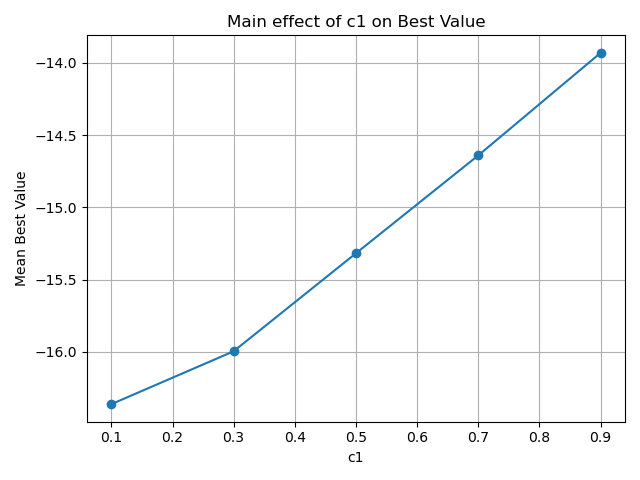
\includegraphics[scale=0.4]{c1_potential10}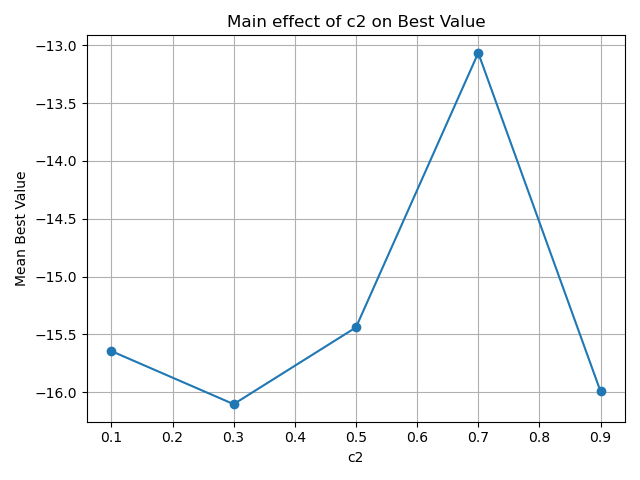
\includegraphics[scale=0.4]{c2_potential10}
\par\end{centering}
\caption{Graphical representation of c1 and c2 for the Potential problem\label{fig:potential}}

\end{figure}
\begin{table}[H]
\caption{Sensitivity analysis of the method parameters for the Rastrigin (Dimension
4)\label{tab:rastrigin}}

\centering{}%
\begin{tabular}{|c|c|c|c|c|c|c|}
\hline 
Rastrigin 4 & Value & Mean & Min & Max & Iters & Main range\tabularnewline
\hline 
\hline 
\multirow{5}{*}{c1} & 0.1 & 2.13634 & 0 & 11.10018 & 150 & \multirow{5}{*}{0.88378}\tabularnewline
\cline{2-6}
 & 0.3 & 1.32079 & 0 & 8.30785 & 150 & \tabularnewline
\cline{2-6}
 & 0.5 & 1.52523 & 0 & 8.1495 & 150 & \tabularnewline
\cline{2-6}
 & 0.7 & 1.25256 & 0 & 7.10786 & 150 & \tabularnewline
\cline{2-6}
 & 0.9 & 1.74395 & 0 & 6.95643 & 150 & \tabularnewline
\hline 
\multirow{5}{*}{c2} & 0.1 & 3.25941 & 0 & 11.10018 & 150 & \multirow{5}{*}{2.44349}\tabularnewline
\cline{2-6}
 & 0.3 & 1.51291 & 0 & 6.55699 & 150 & \tabularnewline
\cline{2-6}
 & 0.5 & 0.81592 & 0 & 5.19549 & 150 & \tabularnewline
\cline{2-6}
 & 0.7 & 1.34782 & 0 & 5.19957 & 150 & \tabularnewline
\cline{2-6}
 & 0.9 & 1.04281 & 0 & 6.60519 & 150 & \tabularnewline
\hline 
\end{tabular}
\end{table}
\begin{figure}[H]
\begin{centering}
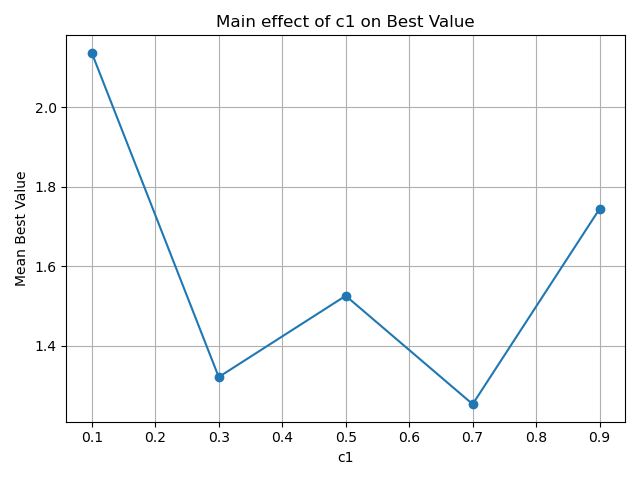
\includegraphics[scale=0.4]{c1_rastrigin4}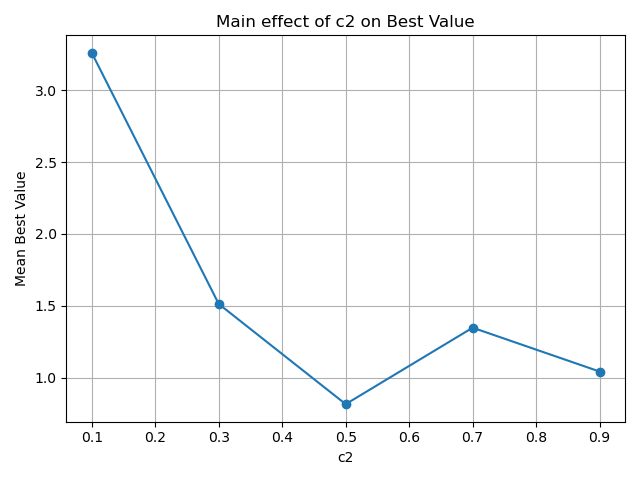
\includegraphics[scale=0.4]{c2_rastrigin4}
\par\end{centering}
\caption{Graphical representation of c1 and c2 for the Rastrigin problem\label{fig:rastrigin}}
\end{figure}
\begin{table}[H]
\caption{Sensitivity analysis of the method parameters for the Test2n problem
(Dimension 4)\label{tab:test2n}}

\centering{}%
\begin{tabular}{|c|c|c|c|c|c|c|}
\hline 
Test2n 4 & Value & Mean & Min & Max & Iters & Main range\tabularnewline
\hline 
\hline 
\multirow{5}{*}{c1} & 0.1 & -146.95432 & -156.66451 & -128.37343 & 150 & \multirow{5}{*}{2.81625}\tabularnewline
\cline{2-6}
 & 0.3 & -146.19977 & -156.66454 & -128.38355 & 150 & \tabularnewline
\cline{2-6}
 & 0.5 & -146.38681 & -156.66442 & -114.25247 & 150 & \tabularnewline
\cline{2-6}
 & 0.7 & -147.60809 & -156.6641 & -114.25223 & 150 & \tabularnewline
\cline{2-6}
 & 0.9 & -149.01602 & -156.66437 & -114.24072 & 150 & \tabularnewline
\hline 
\multirow{5}{*}{c2} & 0.1 & -152.40955 & -156.66454 & -128.39005 & 150 & \multirow{5}{*}{8.94298}\tabularnewline
\cline{2-6}
 & 0.3 & -149.87331 & -156.66447 & -128.38459 & 150 & \tabularnewline
\cline{2-6}
 & 0.5 & -146.48201 & -156.66451 & -114.25223 & 150 & \tabularnewline
\cline{2-6}
 & 0.7 & -143.46657 & -156.66437 & -128.37376 & 150 & \tabularnewline
\cline{2-6}
 & 0.9 & -143.93359 & -156.664 & -114.24072 & 150 & \tabularnewline
\hline 
\end{tabular}
\end{table}
\begin{figure}[H]
\begin{centering}
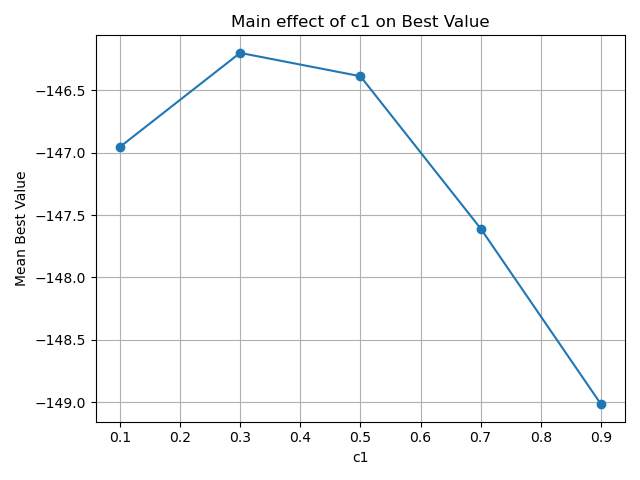
\includegraphics[scale=0.4]{c1_test2n4}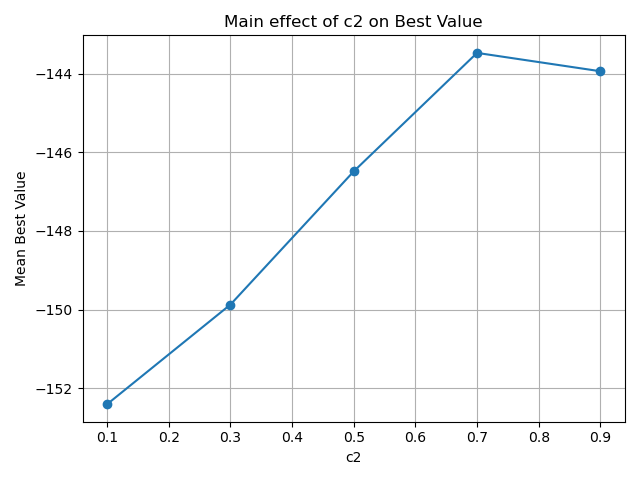
\includegraphics[scale=0.4]{c2_test2n4}
\par\end{centering}
\caption{Graphical representation of c1 and c2 for the Test2n problem\label{fig:test2n}}
\end{figure}
\begin{table}[H]
\caption{Sensitivity analysis of the method parameters for the Rosenbrock problem
(Dimension 4)\label{tab:rosenbrock}}

\centering{}%
\begin{tabular}{|c|c|c|c|c|c|c|}
\hline 
Rosenbrock 4 & Value & Mean & Min & Max & Iters & Main range\tabularnewline
\hline 
\hline 
\multirow{5}{*}{c1} & 0.1 & 35.1061 & 0 & 1354.34838 & 150 & \multirow{5}{*}{30.29039}\tabularnewline
\cline{2-6}
 & 0.3 & 14.66004 & 0 & 1038.60285 & 150 & \tabularnewline
\cline{2-6}
 & 0.5 & 13.3723 & 0 & 593.67884 & 150 & \tabularnewline
\cline{2-6}
 & 0.7 & 9.95311 & 0 & 524.37725 & 150 & \tabularnewline
\cline{2-6}
 & 0.9 & 4.81572 & 0 & 314.03933 & 150 & \tabularnewline
\hline 
\multirow{5}{*}{c2} & 0.1 & 18.00132 & 0 & 1354.34838 & 150 & \multirow{5}{*}{20.91708}\tabularnewline
\cline{2-6}
 & 0.3 & 4.43389 & 0 & 235.09807 & 150 & \tabularnewline
\cline{2-6}
 & 0.5 & 11.78364 & 0 & 593.67884 & 150 & \tabularnewline
\cline{2-6}
 & 0.7 & 18.33745 & 0 & 400.1598 & 150 & \tabularnewline
\cline{2-6}
 & 0.9 & 25.35097 & 0 & 1244.51484 & 150 & \tabularnewline
\hline 
\end{tabular}
\end{table}
\begin{figure}[H]
\begin{centering}
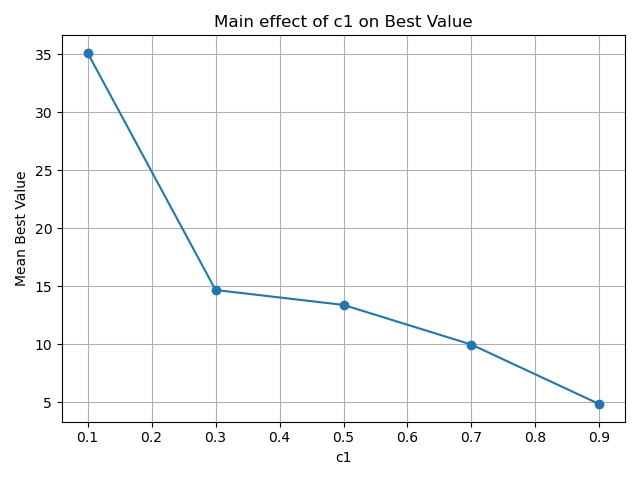
\includegraphics[scale=0.4]{c1_rosenbrock4}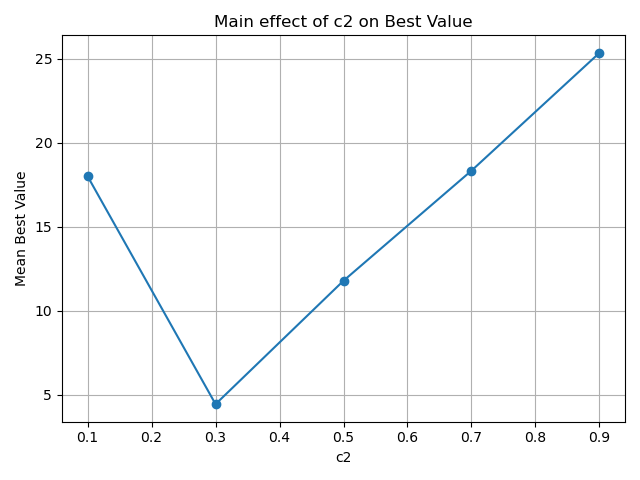
\includegraphics[scale=0.4]{c2_rosenbrock4}
\par\end{centering}
\caption{Graphical representation of c1 and c2 for the Rosenbrock problem\label{fig:rosenbrock}}
\end{figure}

In Potential problem (Table \ref{tab:potential} and Figure \ref{fig:potential}),
the mean best value improves as $c_{1}$ decreases: the Mean Best
moves from \textminus 13.93 ($c_{1}$=0.9) toward \textminus 16.36
($c_{1}$=0.1), with a main effect range of 2.43. This indicates that
for this high-dimensional, strongly multimodal potential, excessive
stochastic dispersion (high $c_{1}$) “blurs” exploitation of promising
areas, whereas mild dispersion supports steady improvement. The impact
of $c_{2}$ is stronger (range 3.04) and non-monotonic: moderate values
around 0.3 yield the best mean performance (\textminus 16.10), while
very low or very high values degrade results. Therefore, in potential
a clear preference emerges for a “moderate” pull toward the best solution
($c_{2}$\ensuremath{\approx}0.3) combined with a low stochastic perturbation
(small $c_{1}$).

In Rastrigin problem (Table \ref{tab:rastrigin} and Figure \ref{fig:rastrigin}),
the behavior differs: $c_{1}$ has a relatively small main effect
(0.88), and the best mean value occurs around $c1$=0.7 (Mean Best\ensuremath{\approx}1.25),
with similar performance at $c_{1}$=0.3. In contrast, $c_{2}$ is
more decisive (range 2.44), with the optimal zone around 0.5 (Mean
Best\ensuremath{\approx}0.82). The Rastrigin function, with its pronounced
symmetric multimodality, benefits from a stronger attraction mechanism
toward the best (moderate $c_{2}$), which helps “lock in” low-value
basins, while a moderate $c_{1}$ maintains enough exploration without
destabilizing convergence. It is notable that the minima are often
0.00, indicating that all combinations can reach the global minimum,
but mean values differentiate reliability and stability.

In Test2n problem (Table \ref{tab:test2n} and Figure \ref{fig:test2n}),
the picture is even clearer in favor of low $c_{2}$: the main effect
of $c_{2}$ is very high (8.94), and the best mean performance appears
at $c_{2}$=0.1 (Mean Best\ensuremath{\approx}\textminus 152.41).
Increasing $c_{2}$ toward 0.7--0.9 significantly worsens mean performance,
although the minima remain near \textminus 156.664 for all settings.
This shows that excessive attraction toward the best induces premature
convergence into local basins and increases performance variability.
$c_{1}$ has a moderate impact (2.82), with a trend suggesting that
larger values (e.g., 0.9) may slightly improve mean performance, likely
by helping to escape narrow polynomial valleys. Overall, in Test2n4,
the guidance is clear: keep $c_{2}$ low and allow $c_{1}$ to be
medium-to-high to maintain consistent solution quality.

In Rosenbrock4 problem (Table \ref{tab:rosenbrock} and Figure \ref{fig:rosenbrock}),
$c_{1}$ has the largest overall effect across all cases (range 30.29),
with a dramatic improvement in mean performance as it increases from
0.1 to 0.9 (Mean Best from \textasciitilde 35.11 to \textasciitilde 4.82).
The Rosenbrock function’s narrow curved valley and anisotropy explain
why stronger stochastic perturbation helps maintain mobility along
the valley and avoid “dead zones” in step progression. $c_{2}$ shows
a U-shaped trend: the best mean performance occurs at 0.3 (Mean Best\ensuremath{\approx}4.43),
while very low or very high $c_{2}$ increases the risk of large outliers,
as seen in maximum values that can spike dramatically. Thus, in {[}rosenbrock4{]},
a high $c_{1}$ is recommended to keep search activity within the
valley, and a moderate $c_{2}$\ensuremath{\approx}0.3 helps avoid
both over-pulling, which can distort the valley geometry, and overly
loose guidance, which delays convergence.

Synthesizing these findings, a consistent tuning pattern emerges:
in highly multimodal landscapes with many symmetric basins such as
Rastrigin, a moderate $c_{2}$ around 0.5 and a moderate $c_{1}$
around 0.3--0.7 minimize mean values and stabilize convergence. In
“parabolic” or polynomial landscapes like Test2n, a low $c_{2}$ and
medium-to-high $c_{1}$ improve stability and mean performance, preventing
premature convergence. In narrow-valley problems like Rosenbrock,
strong $c_{1}$ and moderate $c_{2}$\ensuremath{\approx}0.3 appear
to be the most robust choice. Finally, for dense multimodal potentials
like Potential, the optimal zone tends toward low $c_{1}$ and moderate
$c_{2}$\ensuremath{\approx}0.3, balancing small, targeted jumps with
steady, controlled attraction toward the best.

In practical terms, the ranges that reappear as “safe defaults” are
$c_{2}$ in the moderate range of 0.3--0.5, and $c_{1}$ adapted
to landscape morphology: low for Potential-type landscapes, moderate
for Rastrigin, high for Rosenbrock, and medium-to-high for polynomial
Test2n landscapes. The min/max values per setting highlight the tendency
for extreme deviations when $c_{2}$ is too high or too low especially
in Rosenbrock reinforcing that the ``high $c_{1}$ -- moderate $c_{2}$''
combination is often the most resilient operating point when the goal
is high mean performance rather than isolated best cases.

\subsection{Analysis of Computational Cost and Complexity of the SIOA Algorithm\label{subsec:Computational}}

Figure \ref{fig:computational} illustrates the complexity of the
proposed method, showing the number of objective function calls and
the execution time (in seconds) for problem dimensions ranging from
20 to 260. The experimental settings follow the parameter values specified
in Table \ref{tab:settings}, with the termination criterion based
on the homogeneity of the best value. In addition, a limited local
optimization procedure is applied at a rate of only 0.5\%, enhancing
the exploitation of promising regions in the search space without
significantly affecting the overall global exploration strategy.

More specifically, in the ELLIPSOIDAL problem, the execution time
increases gradually from 0.111 seconds at dimension 20 to 41.714 seconds
at dimension 260, while the corresponding objective function calls
range from 1,398 to 6,457. Similarly, for the ROSENBROCK problem,
the execution time rises from 0.144 seconds at dimension 20 to 40.873
seconds at dimension 260, with the number of calls increasing from
2,83 to 9200. The results indicate that both execution time and the
number of calls grow as the problem dimensionality increases, with
ROSENBROCK generally requiring greater computational effort in higher
dimensions compared to ELLIPSOIDAL. This observation highlights the
sensitivity of the method’s complexity to the nature of the problem,
while also confirming its ability to scale efficiently across a wide
range of search space sizes.

\begin{figure}[H]
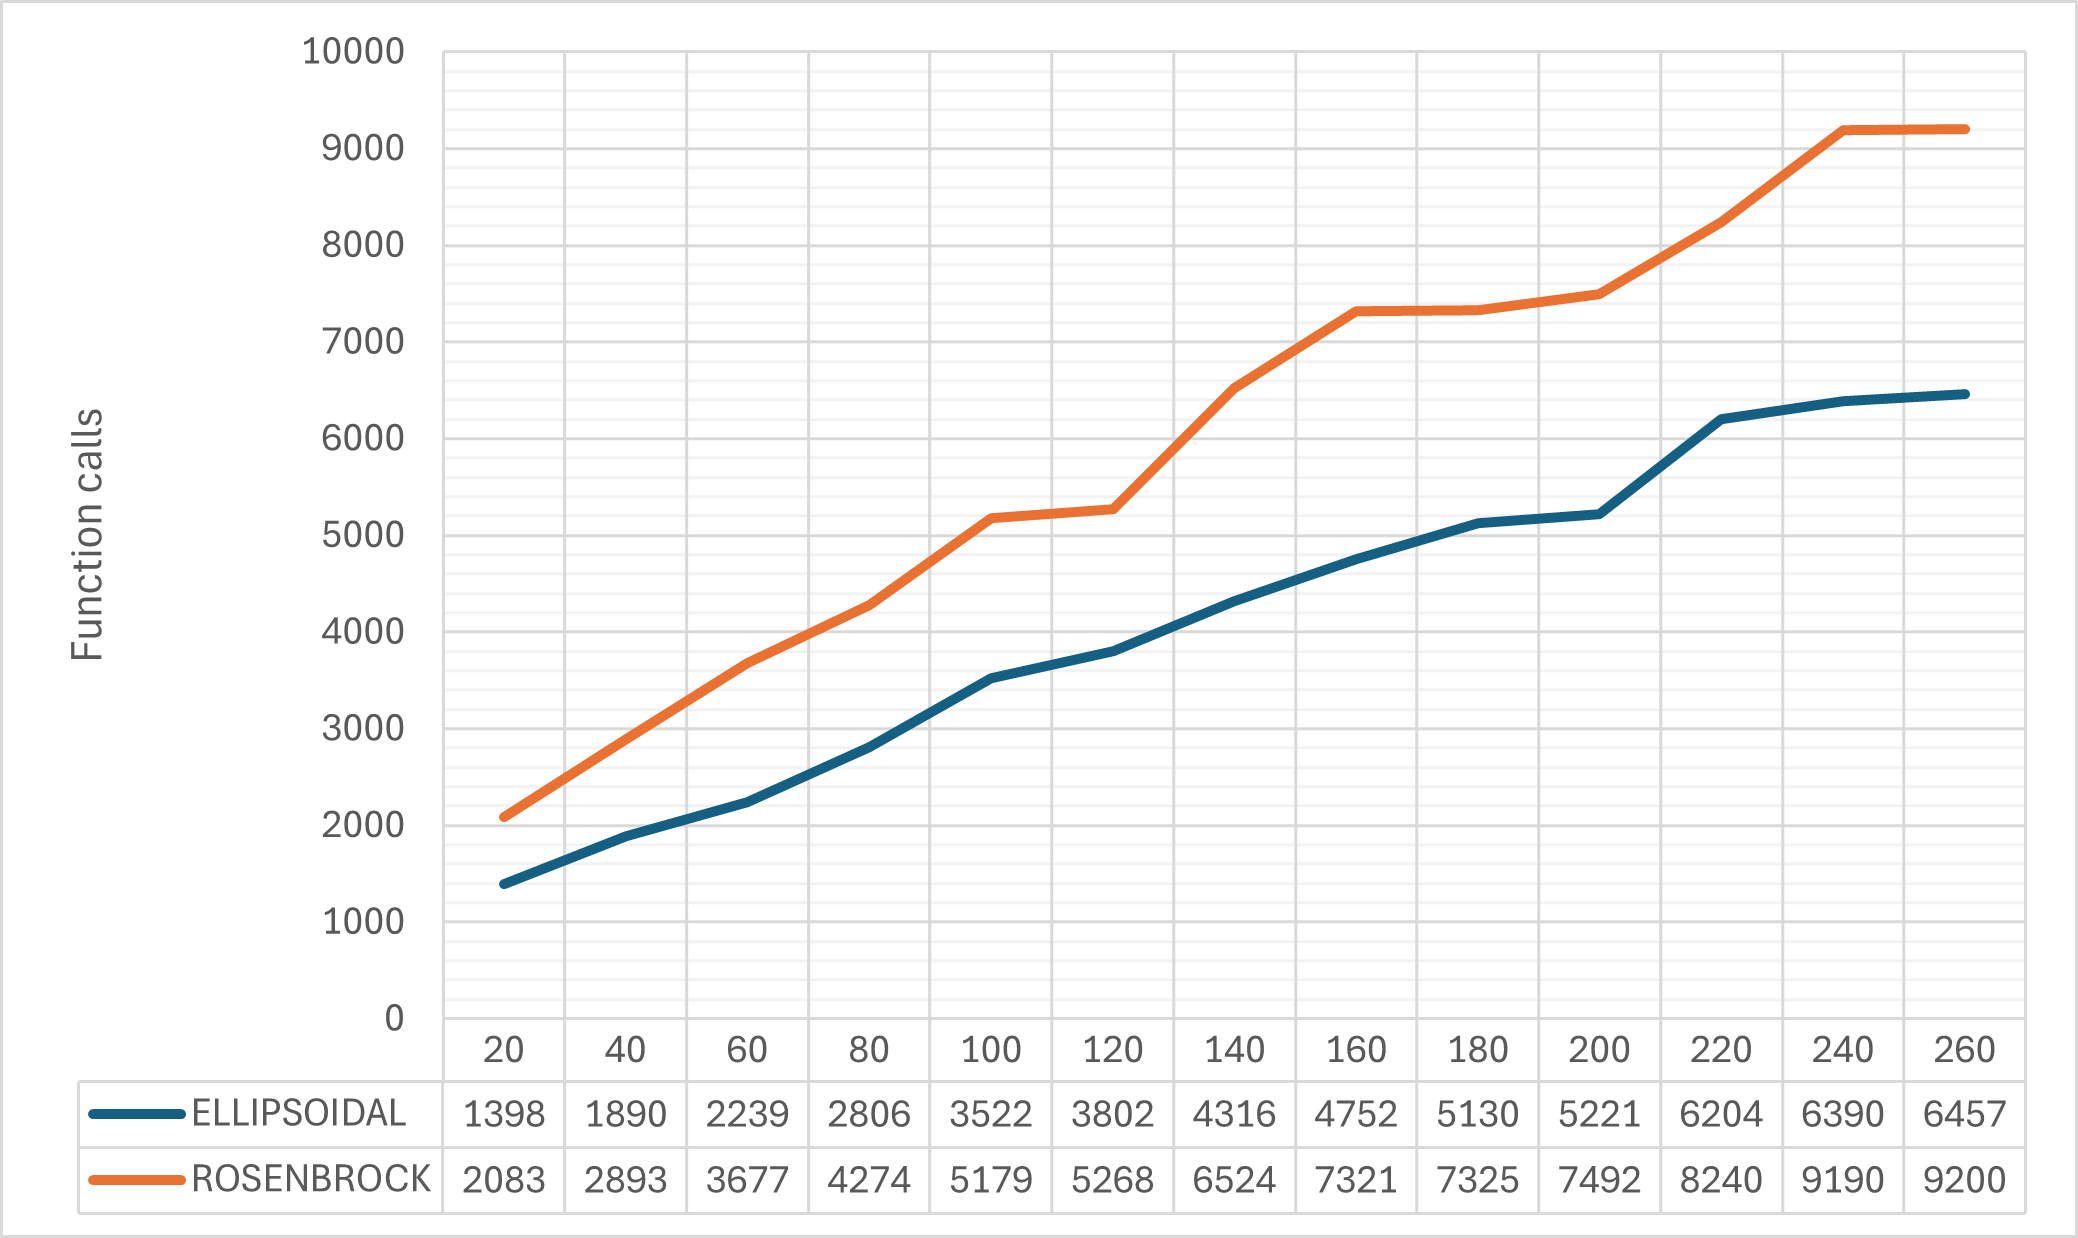
\includegraphics[scale=0.45]{fc}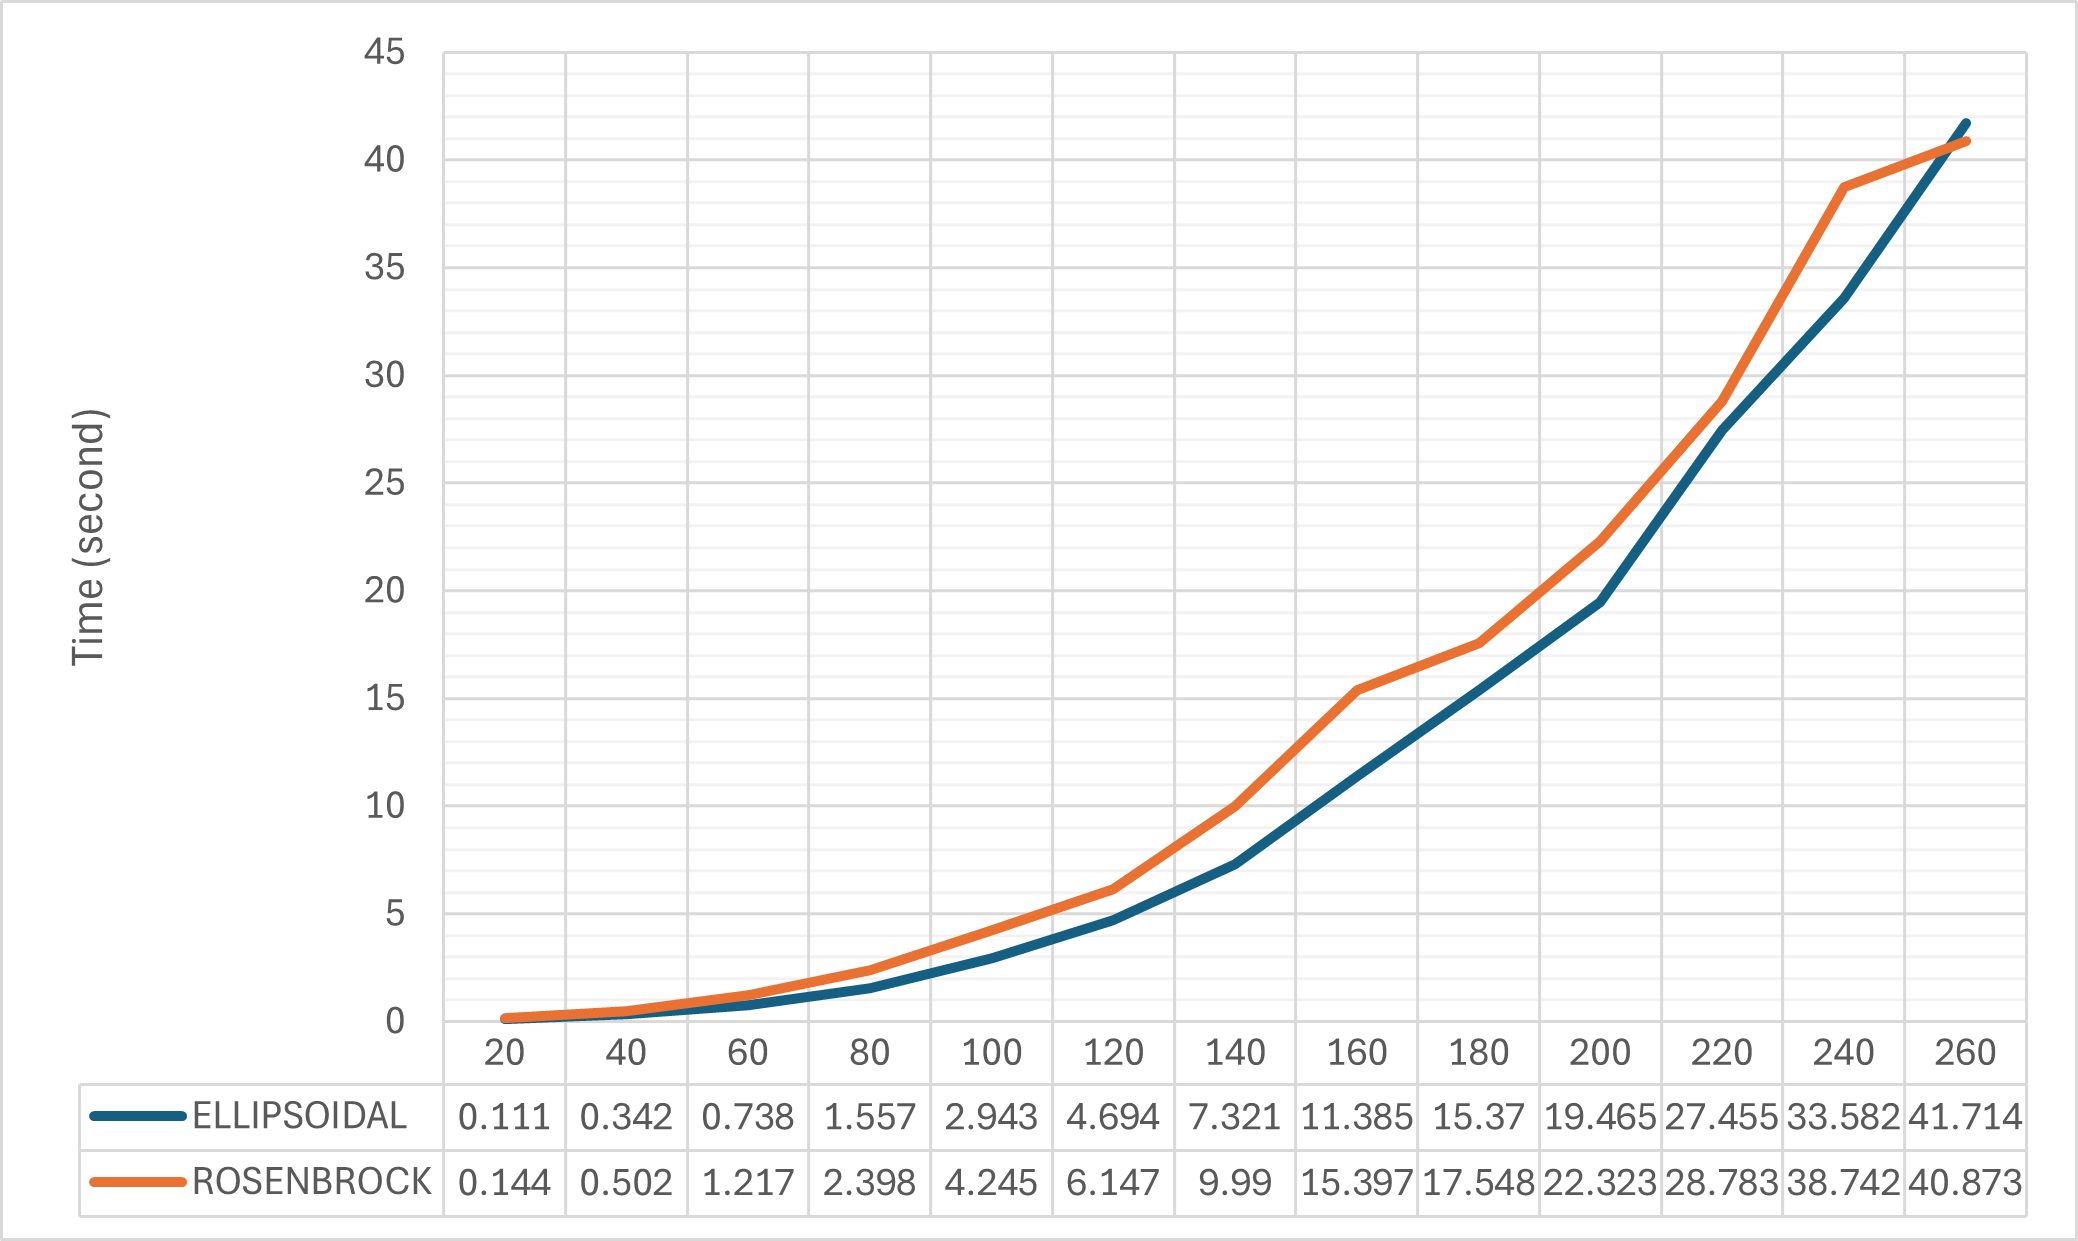
\includegraphics[scale=0.45]{time}

\caption{Computational performance (Calls anad Time) of the proposed method
on ELLIPSOIDAL and ROSENBROCK across dimensions 20-260\label{fig:computational}}
\end{figure}


\section{Conclusions\label{sec:Conclusions}}

Based on the experiments conducted, SIOA proves to be a mature, competitive,
and efficient metaheuristic. In classical benchmark problems, it consistently
outperforms GA, DE, PSO, and ACO in terms of required objective function
calls, while maintaining a high success rate; the overall evaluation
footprint is significantly lower than that of traditional methods,
translating into faster convergence for a given computational budget.
This performance profile supports the view that the biologically inspired
“sporulation--germination” mechanism, combined with self-adaptive
parameter control and similarity-based replacement, provides a tangible
advantage across a wide range of problem types.

The method also demonstrates notable stability: with the parameter
settings of Table \ref{tab:settings}, the best result was reproduced
uniformly in 12 consecutive runs, while local optimization was used
minimally (only 0.5\%), indicating that SIOA’s global search is sufficient
to locate optimal or near-optimal solutions without relying heavily
on exploitation. The algorithm’s core components stochastic perturbation
around an adaptive radius, attraction toward the global best, the
“zero-reset” rule when the optimum lies near the origin, and replacement
through crowding collectively explain both the maintenance of diversity
and the ability to avoid premature convergence.

In more demanding, realistic scenarios with a uniform budget of 150,000
function evaluations and no local optimization, SIOA remains highly
competitive against advanced techniques. Although CMA-ES achieved
the top overall rank, SIOA came very close, with results in certain
cases (e.g., Tersoff Potential and Static Economic Load Dispatch)
approaching the best of the leading competitors. A slightly higher
variance in some less multimodal landscapes limited the mean performance,
highlighting a margin for improvement in stability without undermining
the overall strength of the method.

The scalability analysis shows that both runtime and function evaluations
increase with problem dimension and landscape ruggedness, with problems
such as Rosenbrock generally requiring more computational effort than
smoother ellipsoidal forms an observation consistent with the expected
behavior of metaheuristics in difficult, poorly scaled valleys. In
all cases, SIOA maintains an economical evaluation profile compared
to competing approaches, a feature of direct value in costly simulations.

Overall, the method is realistically ready for application: fast in
terms of evaluations, stable without relying on intensive local search,
and sufficiently flexible to dynamically adapt critical parameters
as the search progresses. At the same time, clear opportunities for
further improvement remain. Realistic next steps include integrating
more specialized, problem-sensitive local optimizers to reduce variance
and improve final accuracy, as well as extending SIOA to constrained,
multi-objective, and large-scale problems, where the combination of
self-adaptation, crowding, and “zero-reset” may yield even greater
benefits. Equally promising are explorations of hybrid versions augmented
with surrogate modeling for expensive problems, further parallelization
and GPU/multi-threaded implementations, the use of restart strategies
and dynamic similarity thresholds, and the development of fully parameter-free
versions with stronger theoretical convergence guarantees. The indicated
extensions to constrained, multi-objective, and large-scale applications,
along with reinforcement via dedicated local search schemes, underscore
SIOA’s realistic potential as a modern foundation for further research
and practical deployment.

\medskip{}


\authorcontributions{V.C. and I.G.T. conducted the experiments, employing all otimization
methods and problems and provided the comparative experiments. D.T.,
A.M.G. and I.G.T.. performed the statistical analysis and prepared
the manuscript. All authors have read and agreed to the published
version of the manuscript.}

\funding{This research received no external funding.}

\institutionalreview{Not Applicable.}

\informedconsent{Not applicable.}

\acknowledgments{This research has been financed by the European Union: Next Generation
EU through the Program Greece 2.0 National Recovery and Resilience
Plan, under the call RESEARCH--CREATE--INNOVATE, project name “iCREW:
Intelligent small craft simulator for advanced crew training using
Virtual Reality techniques” (project code: TAEDK-06195).}

\conflictsofinterest{The authors declare no conflicts of interest.}

\appendixtitles{no}

\begin{adjustwidth}{-\extralength}{0cm}{}

\begin{thebibliography}{999}
\bibitem{key-1}Cauchy, A.-L. (1847). Méthode générale pour la résolution
des systèmes d’équations simultanées. Compte Rendus Hebdomadaires
des Séances de l'Académie des Sciences, 25, 536--538.

\bibitem{key-2}Nocedal, J., \& Wright, S. J. (2006). Numerical Optimization
(2nd ed.). Springer.

\bibitem{key-3}Newton, I. (1736). Method of Fluxions (J. Colson,
Trans.). Henry Woodfall (Original work written in 1671).

\bibitem{key-4}Broyden, C. G. (1970). The convergence of a class
of double-rank minimization algorithms. Journal of the Institute of
Mathematics and Its Applications, 6(1), 76--90. Doi:https://doi.org/10.1093/imamat/6.1.76.

\bibitem{key-5}Fletcher, R. (1970). A new approach to variable metric
algorithms. The Computer Journal, 13(3), 317--322. Doi: https://doi.org/10.1093/comjnl/13.3.317. 

\bibitem{key-6}Goldfarb, D. (1970). A family of variable-metric methods
derived by variational means. Mathematics of Computation, 24(109),
23--26. Doi: https://doi.org/10.2307/2004840.

\bibitem{key-7}Shanno, D. F. (1970). Conditioning of quasi-Newton
methods for function minimization. Mathematics of Computation, 24(111),
647--656.Doi: https://doi.org/10.2307/2004843.

\bibitem{key-8}Gauss, C. F. (1809). Theoria motus corporum coelestium
in sectionibus conicis solem ambientium. Hamburg: Friedrich Perthes
und I. H. Besser.

\bibitem{key-9}Metropolis, N., \& Ulam, S. (1949). The Monte Carlo
method. Journal of the American Statistical Association, 44(247),
335--341. Doi: https://doi.org/10.1080/01621459.1949.10483310

\bibitem{key-10}Kroese, D. P., Brereton, T., Taimre, T., \& Botev,
Z. I. (2014). Why the Monte Carlo method is so important today. Wiley
Interdisciplinary Reviews: Computational Statistics, 6(6), 386--392.
Doi:https://doi.org/10.1002/wics.1314.

\bibitem{key-11}Kirkpatrick, S., Gelatt, C. D., \& Vecchi, M. P.
(1983). Optimization by simulated annealing. Science, 220(4598), 671--680.
Doi: https://doi.org/10.1126/science.220.4598.671.

\bibitem{key-12}Aarts, E., \& Korst, J. (1989). Simulated Annealing
and Boltzmann Machines: A stochastic approach to combinatorial optimization
and neural computing. Wiley.

\bibitem{key-13}Wenzel, W., \& Hamacher, K. (1999). Stochastic tunneling
approach for global minimization of complex potential energy landscapes.
Physical Review Letters, 82(15), 3003--3007. Doi: https://doi.org/10.1103/PhysRevLett.82.3003.

\bibitem{key-14}Geyer, C. J. (1991). Markov chain Monte Carlo maximum
likelihood. In Computing Science and Statistics: Proceedings of the
23rd Symposium on the Interface (Vol. 23, pp. 156--163).

\bibitem{key-15}Holland, J. H. (1975). Adaptation in natural and
artificial systems. University of Michigan Press.

\bibitem{key-16}Mitchell, M. (1998). An introduction to genetic algorithms.
MIT Press.

\bibitem{key-17}Storn, R., \& Price, K. (1997). Differential evolution
-- A simple and efficient heuristic for global optimization over
continuous spaces. Journal of Global Optimization, 11(4), 341--359.
Doi: https://doi.org/10.1023/A:1008202821328.

\bibitem[(2022)]{key-100}Charilogis, V., Tsoulos, I.G.,Tzallas, A.,Karvounis,
E. (2022). Modifications for the Differential Evolution Algorithm.
Symmetry ,2022,14,447. Doi: https://doi.org/10.3390/sym14030447

\bibitem[(2023)]{key-101}Charilogis, V.; Tsoulos, I.G.(2023). A Parallel
Implementation of the Differential Evolution Method. Analytics, 2,
17--30. 

\bibitem{key-18}Simon, D. (2008). Biogeography-based optimization.
IEEE Transactions on Evolutionary Computation, 12(6), 702--713. Doi:
https://doi.org/10.1109/TEVC.2008.919004.

\bibitem{key-19}Reynolds, R. G. (1994). An introduction to cultural
algorithms. In Proceedings of the Third Annual Conference on Evolutionary
Programming (pp. 131--139). World Scientific. ISBN: 9789810218635.

\bibitem{key-21}Torczon, V. (1997). On the convergence of pattern
search algorithms. SIAM Journal on Optimization, 7(1), 1--25.Doi:
https://doi.org/10.1137/S1052623493250780.

\bibitem{key-22}Kolda, T. G., Lewis, R. M., \& Torczon, V. (2003).
Optimization by direct search: New perspectives on some classical
and modern methods. SIAM Review, 45(3), 385--482. Doi: https://doi.org/10.1137/S003614450242889.

\bibitem{key-23}Nelder, J. A., \& Mead, R. (1965). A simplex method
for function minimization. The Computer Journal, 7(4), 308--313.
Doi: https://doi.org/10.1093/comjnl/7.4.308.

\bibitem{key-24}Matheron, G. (1963). Principles of geostatistics.
Economic Geology, 58(8), 1246--1266. Doi: https://doi.org/10.2113/gsecongeo.58.8.1246.

\bibitem{key-25}Sacks, J., Welch, W. J., Mitchell, T. J., \& Wynn,
H. P. (1989). Design and analysis of computer experiments. Statistical
Science, 4(4), 409--423. Doi: https://doi.org/10.1214/ss/1177012413.

\bibitem{key-26}Hardy, R. L. (1971). Multiquadric equations of topography
and other irregular surfaces. Journal of Geophysical Research, 76(8),
1905--1915. Doi:https://doi.org/10.1029/JB076i008p01905.

\bibitem{key-27}Powell, M. J. D. (1987). Radial basis functions for
multivariable interpolation: A review. In Algorithms for Approximation
(pp. 143--167). Clarendon Press.

\bibitem{key-28}Wiener, N. (1938). The homogeneous chaos. American
Journal of Mathematics, 60(4), 897--936. Doi:https://doi.org/10.2307/2371268.

\bibitem{key-29}Mockus, J., Tiesis, V., \& Zilinskas, A. (1978).
The application of Bayesian methods for seeking the extremum. In Towards
Global Optimization (Vol. 2, pp. 117--129). North-Holland.

\bibitem{key-30}Han, S. P. (1977). A globally convergent method for
nonlinear programming. Journal of Optimization Theory and Applications,
22(3), 297--309. Doi:https://doi.org/10.1007/BF00932869.

\bibitem{key-31}Conn, A. R., Scheinberg, K., \& Vicente, L. N. (2009).
Introduction to Derivative-Free Optimization. SIAM. Doi: https://doi.org/10.1137/1.9780898718768.

\bibitem{key-32}Powell, M. J. D. (2004). The NEWUOA software for
unconstrained optimization without derivatives. Technical Report DAMTP
2004/NA05, University of Cambridge.

\bibitem{key-33}Rockafellar, R. T. (1970). Convex Analysis. Princeton
University Press.

\bibitem{key-34}Karmarkar, N. (1984). A new polynomial-time algorithm
for linear programming. Combinatorica, 4(4), 373--395. Doi: https://doi.org/10.1007/BF02579150.

\bibitem{key-35}Shor, N. Z. (1985). Minimization Methods for Non-Differentiable
Functions. Springer.

\bibitem{key-36}Kelley, J. E. (1960). The cutting-plane method for
solving convex programs. Journal of the Society for Industrial and
Applied Mathematics, 8(4), 703--712. Doi: https://doi.org/10.1137/0105057.

\bibitem{key-37}Benders, J. F. (1962). Partitioning procedures for
solving mixed-variables programming problems. Numerische Mathematik,
4, 238--252. Doi: https://doi.org/10.1007/BF01386316.

\bibitem{key-38}Dantzig, G. B., \& Wolfe, P. (1960). Decomposition
principle for linear programs. Operations Research, 8(1), 101--111.Doi:
https://doi.org/10.1287/opre.8.1.101.

\bibitem{key-39}Held, M., \& Karp, R. M. (1971). The traveling-salesman
problem and minimum spanning trees. Operations Research, 18(6), 1138--1162.
Doi: https://doi.org/10.1287/opre.18.6.1138.

\bibitem{key-40}Jones, D. R., Perttunen, C. D., \& Stuckman, B. E.
(1993). Lipschitzian optimization without the Lipschitz constant.
Journal of Optimization Theory and Applications, 79(1), 157--181.
Doi: https://doi.org/10.1007/BF00941892.

\bibitem{key-43}Land, A. H., \& Doig, A. G. (1960). An automatic
method for solving discrete programming problems. Econometrica, 28(3),
497--520. Doi: https://doi.org/10.2307/1910129.

\bibitem{key-44}Moore, R. E. (1966). Interval Analysis. Englewood
Cliffs, NJ: Prentice-Hall.

\bibitem{key-45}Miller, G. F., Todd, P. M., \& Hegde, S. U. (1989).
Designing neural networks using genetic algorithms. In Proceedings
of the Third International Conference on Genetic Algorithms (pp. 379--384).
Morgan Kaufmann.

\bibitem{key-46}Sutton, R. S. (1988). Learning to predict by the
methods of temporal differences. Machine Learning, 3, 9--44. Doi:
https://doi.org/10.1007/BF00115009.

\bibitem{key-47}Mnih, V., et al. (2015). Human-level control through
deep reinforcement learning. Nature, 518(7540), 529--533. Doi: https://doi.org/10.1038/nature14236.

\bibitem{key-48}Kennedy, J., \& Eberhart, R. (1995). Particle swarm
optimization. In Proceedings of ICNN'95 - International Conference
on Neural Networks (Vol. 4, pp. 1942--1948). IEEE. Doi: https://doi.org/10.1109/ICNN.1995.488968

\bibitem{key-49}Dorigo, M. (1992). Optimization, learning and natural
algorithms (Doctoral dissertation, Politecnico di Milano).

\bibitem{key-50}Karaboga, D. (2005). An idea based on honey bee swarm
for numerical optimization (Technical Report TR06). Erciyes University,
Engineering Faculty, Computer Engineering Department.

\bibitem{key-51}Yang, X. S. (2008). Nature-inspired metaheuristic
algorithms (1st ed.). Luniver Press.

\bibitem{key-52}Zhou, C. G., \& Gen, M. (1999). A new approach to
global optimization: Simulated crystallization. IEEE Transactions
on Systems, Man, and Cybernetics - Part A: Systems and Humans, 29(4),
429--435. Doi: https://doi.org/10.1109/3468.769584.

\bibitem{key-53}Rashedi, E., Nezamabadi-Pour, H., \& Saryazdi, S.
(2009). GSA: A gravitational search algorithm. Information Sciences,
179(13), 2232--2248. Doi: https://doi.org/10.1016/j.ins.2009.01.010.

\bibitem{key-54}Birbil, S. İ., \& Fang, S. C. (2003). An electromagnetism-like
mechanism for global optimization. Journal of Global Optimization,
25, 263--282.Doi: https://doi.org/10.1023/A:1022472315277.

\bibitem{key-55}Kaveh, A., \& Talatahari, S. (2010). A novel heuristic
optimization method: Charged system search. Acta Mechanica, 213(3--4),
267--289. Doi: https://doi.org/10.1007/s00707-009-0270-4.

\bibitem{key-56}Jang, J.-S. R. (1993). ANFIS: Adaptive-network-based
fuzzy inference system. IEEE Transactions on Systems, Man, and Cybernetics,
23(3), 665--685. Doi: https://doi.org/10.1109/21.256541.

\bibitem{key-57}Moscato, P. (1989). On Evolution, Search, Optimization,
Genetic Algorithms and Martial Arts: Towards Memetic Algorithms (Technical
Report C3P 826). California Institute of Technology, Pasadena, CA.

\bibitem{key-58}Reynolds, R. G. (1994). An introduction to cultural
algorithms. Proceedings of the Third Annual Conference on Evolutionary
Programming, 131--139.

\bibitem{key-59}Koza, J. R. (1992). Genetic programming: On the programming
of computers by means of natural selection. MIT Press.

\bibitem{key-60}Dasgupta, D., \& Forrest, S. (1996). Artificial immune
systems in industrial applications. In Proceedings of the Second International
Conference on Intelligent Processing and Manufacturing of Materials
(Vol. 1, pp. 257--267). IEEE. Doi: https://doi.org/10.1109/IPMM.1997.618940

\bibitem{key-61}Passino, K. M. (2002). Biomimicry of bacterial foraging
for distributed optimization and control. IEEE Control Systems Magazine,
22(3), 52--67. Doi: https://doi.org/10.1109/MCS.2002.1004010.

\bibitem{key-62}Mehrabian, A. R., \& Lucas, C. (2006). A novel numerical
optimization algorithm inspired from weed colonization. Ecological
Informatics, 1(4), 355--366. Doi: https://doi.org/10.1016/j.ecoinf.2006.07.003.

\bibitem{key-64}Geem, Z. W., Kim, J. H., \& Loganathan, G. V. (2001).
A new heuristic optimization algorithm: Harmony search. Simulation,
76(2), 60--68. Doi: https://doi.org/10.1177/003754970107600201.

\bibitem{key-65}Rao, R. V., Savsani, V. J., \& Vakharia, D. P. (2011).
Teaching--learning-based optimization: A novel method for constrained
mechanical design optimization problems. Computer-Aided Design, 43(3),
303--315. Doi: https://doi.org/10.1016/j.cad.2010.12.015.

\bibitem{key-66}Shah-Hosseini, H. (2012). The intelligent water drops
algorithm: A nature-inspired swarm-based optimization algorithm. International
Journal of Bio-Inspired Computation, 4(4), 245--260. Doi: https://doi.org/10.1504/IJBIC.2012.048490.

\bibitem{key-67}Mahdavi, M., Fesanghary, M., \& Damangir, E. (2010).
An improved harmony search algorithm for solving optimization problems.
Applied Mathematics and Computation, 188(2), 1567--1579.

\bibitem{key-68}Kashan, M. H. (2014). League championship algorithm
(LCA): An algorithm for global optimization inspired by sport championships.
Applied Soft Computing, 16, 171--200. Doi: https://doi.org/10.1016/j.asoc.2013.12.005.

\bibitem{key-69}Atashpaz-Gargari, E., \& Lucas, C. (2007). Imperialist
competitive algorithm: An algorithm for optimization inspired by imperialistic
competition. In 2007 IEEE Congress on Evolutionary Computation (pp.
4661--4667). IEEE. Doi: https://doi.org/10.1109/CEC.2007.4425083.

\bibitem{key-70}Han, K. H., \& Kim, J. H. (2004). Quantum-inspired
evolutionary algorithm for a class of combinatorial optimization.
IEEE Transactions on Evolutionary Computation, 6(6), 580--593. Doi:
https://doi.org/10.1109/TEVC.2004.831456.

\bibitem{key-71}Lam, A. Y. S., \& Li, V. O. K. (2010). Chemical-reaction-inspired
metaheuristic for optimization. IEEE Transactions on Evolutionary
Computation, 14(3), 381--399. Doi: https://doi.org/10.1109/TEVC.2009.2033583.

\bibitem{key-72}Tung, Y. C., \& Quek, C. (2004). Social cognitive
optimization: A particle swarm inspired approach. In Proceedings of
the IEEE Congress on Evolutionary Computation (Vol. 2, pp. 2292--2299).
IEEE. Doi: https://doi.org/10.1109/CEC.2004.1331147.

\bibitem[(2020)]{key-107}Lam, A. (2020). BFGS in a Nutshell: An Introduction
to Quasi-Newton Methods Demystifying the inner workings of BFGS optimization.
Towards Data Science.

\bibitem[(2022)]{key-108}Charilogis, V. \& Tsoulos, I.G.(2022).Toward
an Ideal Particle Swarm Optimizer for Multidimensional Functions.
Information, 13, 217.Doi: https://doi.org/10.3390/info13050217

\bibitem[(2025)]{key-109}Gianni, A.M.; Tsoulos, I.G.;Charilogis,
V.; Kyrou, G. (2025). Enhancing Differential Evolution: A Dual Mutation
Strategy with Majority Dimension Voting and New Stopping Criteria.
Symmetry 2025, 17, 844. https://doi.org/10.3390/sym17060844

\bibitem[(2023)]{key-106}Siarry, P., Berthiau, G., Durdin, F., \&
Haussy, J. (1997). Enhanced simulated annealing for globally minimizing
functions of many-continuous variables. ACM Transactions on Mathematical
Software (TOMS), 23(2), 209-228

\bibitem[(2019)]{key-110}Koyuncu, H., \& Ceylan, R. (2019). A PSO
based approach: Scout particle swarm algorithm for continuous global
optimization problems. Journal of Computational Design and Engineering,
6(2), 129-142.

\bibitem[(2021)]{key-111}LaTorre, A., Molina, D., Osaba, E., Poyatos,
J., Del Ser, J., \& Herrera, F. (2021). A prescription of methodological
guidelines for comparing bio-inspired optimization algorithms. Swarm
and Evolutionary Computation, 67, 100973.

\bibitem[(2003)]{key-112}Gaviano, M., Kvasov, D. E., Lera, D., \&
Sergeyev, Y. D. (2003). Algorithm 829: Software for generation of
classes of test functions with known local and global minima for global
optimization. ACM Transactions on Mathematical Software (TOMS), 29(4),
469-480.

\bibitem[(1924)]{key-113}Jones, J. E. (1924). On the determination
of molecular fields.---II. From the equation of state of a gas. Proceedings
of the Royal Society of London. Series A, Containing Papers of a Mathematical
and Physical Character, 106(738), 463-477.

\bibitem[(1992)]{key-114}Zabinsky, Z. B., Graesser, D. L., Tuttle,
M. E., \& Kim, G. I. (1992). Global optimization of composite laminates
using improving hit and run. In Recent advances in global optimization
(pp. 343-368).

\bibitem[(2003)]{key-115}Tsoulos, I.G., Charilogis, V., Kyrou, G.,
Stavrou, V.N. \& Tzallas,A. (2025). OPTIMUS: A Multidimensional Global
Optimization Package. Journal of Open Source Software, 10(108), 7584.
Doi: https://doi.org/10.21105/joss.07584.

\bibitem[(1937)]{key-200}Friedman, M. (1937). The use of ranks to
avoid the assumption of normality implicit in the analysis of variance.
Journal of the american statistical association, 32(200), 675-701.
Doi: https://doi.org/10.1080/01621459.1937.105035

\bibitem[(2012)]{key-1}Lee, Y., Filliben, J., Micheals,R. \& Phillips
,J. (2012). Sensitivity Analysis for Biometric Systems: A Methodology
Based on Orthogonal Experiment Designs. National Institute of Standards
and Technology Gaithersburg (NISTIR), MD 20899. Doi: http://dx.doi.org/10.6028/NIST.IR.7855

\end{thebibliography}

\end{adjustwidth}{}
\end{document}
